\documentclass[manuscript, screen]{timtm}

\makeatletter%
\@ifclassloaded{acmart}%
  {\AtBeginDocument{%
  \providecommand\BibTeX{{%
   \normalfont B\kern-0.5em{\scshape i\kern-0.25em b}\kern-0.8em\TeX}}}}%
  {\AtBeginDocument{%
  \providecommand\BibTeX{{%
   \rm B\kern-.05em{\sc i\kern-.025em b}\kern-.08em\TeX}}}}%
\makeatother%

\setcopyright{rightsretained}
\copyrightyear{2026}

%% If you are going to include source code (or code snippets) you can use minted in a listings environment
% This is also necessary for the For DIVA page
\usepackage{listings}		    %% For source code listing

%% The following are needed for generating the DiVA page(s)
\usepackage[force-eol=true]{scontents}              %% Needed to save lang, abstract, and keywords
\usepackage{pgffor}                 %% includes the foreach loop

% The following is needed in conjunction with generating the DiVA data with abstracts and keywords using the scontents package and a modified listings environment
\makeatletter
\let\verbatimsc\@undefined
\let\endverbatimsc\@undefined
\lst@AddToHook{Init}{\hyphenpenalty=50\relax}
\makeatother


\lstnewenvironment{verbatimsc}
    {
    \lstset{%       \sffamily\tiny
        basicstyle=\linespread{1}\ttfamily\tiny,
        backgroundcolor=\color{white},
        %basicstyle=\tiny,
        columns=fullflexible,           %% for abstracts, needs to be set for pdfLaTeX
        %columns=[l]fixed,
        language=[LaTeX]TeX,
        %numbers=left,
        %numberstyle=\tiny\color{gray},
        keywordstyle=\color{red},
        breaklines=true,                 % sets automatic line breaking
        breakatwhitespace=true,          % sets if automatic breaks should only happen at whitespace
        %keepspaces=false,
        breakindent=0em,
        %fancyvrb=true,
        frame=none,                     % turn off any box
        postbreak={}                    % turn off any hook arrow for continuation
    }
}{}

%% Add some more keyowrds to bring out the structure more
\lstdefinestyle{[LaTeX]TeX}{
morekeywords={begin, todo, textbf, textit, texttt}
}

\lstset{
  literate={ä}{{\"a}}1
           {ö}{{\"o}}1
           {ü}{{\"u}}1
           {å}{{\aa}}1
           {Ä}{{\"A}}1
           {Ö}{{\"O}}1
           {Ü}{{\"U}}1
           {Å}{{\AA}}1
}

% for experiments with new cover
\usepackage{eso-pic}
\usepackage[absolute,overlay]{textpos}

\usepackage{tikz}
\usepackage{colortbl}
\usetikzlibrary{arrows,decorations.pathmorphing,backgrounds,fit,positioning, decorations.pathreplacing, calc,shapes}
\usepackage{graphicx}
\graphicspath{{figures/}{./figures/}{../figures/}}

\input{lib/kthcolors}

% Draft toggle for Overleaf.
% Set \fullfiguresfalse for a lighter compile with only the core figures.
% Set \fullfigurestrue to include the full figure set.
\newif\iffullfigures
\fullfiguresfalse

\makeatletter%
\@ifclassloaded{acmart}%
{%
\newcommand{\alttitle}[1]{}
\newcommand{\altsubtitle}[1]{}
\newenvironment{swedishabstract}{}{}
\newcommand{\SwedishKeywords}[1]{}
}{%
\newcommand{\showISBNx}{}
\newcommand{\showISBNxiii}{}
}%
\makeatother%

\begin{document}
%% Information for inside title page

\authorsLastname{Cvetkovic}
\authorsFirstname{Mihailo}
\firstemail{mihailoc@ug.kth.se}
\kthid{ADD-KTH-ID}
\authorsSchool{\schoolAcronym{EECS}}
\authorCityCountryDate{\MONTH\enspace\the\year}

% Leave these empty for a single-author thesis.
\secondAuthorsLastname{}
\secondAuthorsFirstname{}
\secondemail{}
\secondkthid{}
\secondAuthorsSchool{}

\supervisorAsLastname{TO-BE-COMPLETED}
\supervisorAsFirstname{Supervisor}
\supervisorAsEmail{supervisor@kth.se}
\supervisorAsKTHID{ADD-KTH-ID}
\supervisorAsSchool{\schoolAcronym{EECS}}
\supervisorAsDepartment{TO-BE-COMPLETED}

\supervisorBsLastname{}
\supervisorBsFirstname{}
\supervisorBsEmail{}
\supervisorBsKTHID{}
\supervisorBsSchool{}
\supervisorBsDepartment{}

\supervisorCsLastname{}
\supervisorCsFirstname{}
\supervisorCsEmail{}
\supervisorCsOrganization{}

\examinersLastname{TO-BE-COMPLETED}
\examinersFirstname{Examiner}
\examinersEmail{examiner@kth.se}
\examinersKTHID{ADD-KTH-ID}
\examinersSchool{\schoolAcronym{EECS}}
\examinersDepartment{TO-BE-COMPLETED}

\hostcompany{}

\date{June 2026}

\courseCycle{2}
\courseCode{DA232X}
\courseCredits{30.0}

\programcode{TIMTM}
\degreeName{Master of Science}
\subjectArea{Media Technology}
\secondSubjectArea{Computer Science and Engineering}

\nationalsubjectcategories{10201, 10209}

\presentationDateAndTimeISO{2026-00-00 00:00}
\presentationLanguage{eng}
\presentationRoom{TO-BE-COMPLETED}
\presentationAddress{Isafjordsgatan 22 (Kistagången 16)}
\presentationCity{Stockholm}

\opponentsNames{TO-BE-COMPLETED}
\trita{TRITA -- EECS-EX}{2026:0000}


\title[Anomaly Detection in District Heating Substations]{Anomaly Detection in District Heating Substations Using Reconstruction-Based Models}
\alttitle{Anomalidetektion i fj\"arrv\"armecentraler med rekonstruktionsbaserade modeller}

\makeatletter
\author{\@authorsFirstname\space\@authorsLastname}
\email{\@email}
\if\relax\detokenize\expandafter{\@secondAuthorsFirstname}\relax\else
\author{\@secondAuthorsFirstname\space\@secondAuthorsLastname}
\email{\@secondemail}
\fi
\affiliation{%
  \institution{KTH Royal Institute of Technology, School of Electrical Engineering and Computer Science}
  \city{Stockholm}
  \country{Sweden}
  \postcode{SE 100 44}
}
\makeatother

\begin{abstract}
\begin{scontents}[store-env=abstracts,print-env=false]
This thesis investigates anomaly detection in a small district-heating network using historical operational data from multiple consumer substations. The work starts from the HEAT paper as a methodological reference, but adapts the approach to a setting with fewer substations, longer historical coverage, and limited fault labels. The main method is a reconstruction-based anomaly detector that models 24-hour windows of supply temperature, return temperature, and derived flow. The study compares engineering baselines, thresholding rules, dominant-feature attribution, and clustering-based interpretation in order to identify anomaly candidates that can be reviewed with domain experts and later applied to live operational data.
\end{scontents}
\end{abstract}

\begin{swedishabstract}
\begin{scontents}[store-env=abstracts,print-env=false]
Detta examensarbete unders\"oker anomalidetektion i ett litet fj\"arrv\"armen\"at med hj\"alp av historiska driftsdata fr\aa n flera kundcentraler. Arbetet utg\aa r fr\aa n HEAT-artikeln som metodologisk referens, men anpassar angreppss\"attet till en situation med f\"arre undercentraler, l\"angre historisk t\"ackning och begr\"ansad tillg\aa ng till felm\"arkta data. Huvudmetoden \"ar en rekonstruktionsbaserad anomalidetektor som modellerar 24-timmarsf\"onster av framledningstemperatur, returtemperatur och h\"arlett fl\"ode. Studien j\"amf\"or ingenj\"orsm\"assiga baslinjer, tr\"oskelv\"ardesmetoder, dominant-funktionsattribuering och klusterbaserad tolkning f\"or att identifiera anomalikandidater som kan granskas tillsammans med dom\"anexperter och senare anv\"andas p\aa\ live-data.
\end{scontents}
\end{swedishabstract}

\keywords{district heating, anomaly detection, autoencoder, reconstruction error, time-series analysis}
\SwedishKeywords{fj\"arrv\"arme, anomalidetektion, autoencoder, rekonstruktionsfel, tidsserieanalys}

\pagenumbering{alph}
% Disable the template cover in the working draft: it is the main source of
% Overleaf compatibility issues and adds compile overhead without affecting
% the thesis content under review.
% \kthcover
\titlepage

\pagenumbering{arabic}
\setcounter{page}{1}
\maketitle

\tableofcontents
\clearpage

\section{Introduction}

District-heating substations operate continuously and generate large volumes of time-series data, but real fault labels are often sparse or unavailable. This creates a practical detection problem: operators still need a way to identify unusual operating periods, even when a supervised classification setup is not possible. The aim of this thesis is therefore to build and evaluate an anomaly-detection pipeline that can identify physically interpretable abnormal behavior in district-heating substations using historical data and later be applied to live data.

The work is motivated by the HEAT paper, which combines encoder-based representation learning and clustering for fault detection in district-heating substations. However, the available KTH thesis dataset differs in two important ways. First, the network is much smaller, which weakens the statistical value of peer-group clustering. Second, the historical coverage is much longer, which makes per-substation temporal modeling more promising than network-wide peer comparison alone. Because of this, the thesis focuses primarily on reconstruction-based anomaly detection and treats clustering as a supporting interpretation tool rather than the central detection mechanism.

The main research question is:

\begin{quote}
Can reconstruction-based anomaly detection on supply temperature, return temperature, and derived flow identify interpretable abnormal operating periods in a small district-heating network?
\end{quote}

The thesis also addresses the following supporting questions:

\begin{itemize}
\item How should the derived flow feature be handled when small temperature differences cause numerical instability?
\item How does a reconstruction-based detector compare with a simple engineering low delta-T baseline?
\item What is the effect of threshold choice on the number and type of detected anomalies?
\item Can clustering still help as an interpretation layer when the number of substations is small?
\end{itemize}

The rest of the thesis is organized as follows. Chapter~2 reviews the relevant background and the HEAT paper. Chapter~3 describes the available datasets and preprocessing assumptions. Chapter~4 presents the anomaly-detection methodology. Chapter~5 summarizes the experimental results. Chapter~6 discusses interpretation, limitations, and implications for live deployment. Chapter~7 concludes the thesis and outlines future work.

\section{Background}

\subsection{District-heating anomaly detection}

District-heating systems are monitored through temperature, flow, and power-related signals that reflect both thermal performance and hydraulic behavior. In practice, low supply-return temperature difference is often used as a first engineering warning sign because it may indicate poor heat extraction, inefficient operation, or high return-temperature behavior. However, low delta-T only captures one narrow anomaly type and cannot describe all abnormal operating patterns.

\subsection{HEAT paper as reference}

The HEAT paper proposes a hierarchical-constrained, encoder-assisted clustering approach for fault detection in district-heating substations. Its main idea is to learn compact representations of time-series behavior and then use clustering to approximate peer groups for local comparison. This is well suited to a large network with many substations, where peer comparison can be statistically meaningful.

In this thesis, HEAT remains the main methodological reference. The adaptation is necessary because the available dataset has far fewer consumer sheets than the HEAT case study. The practical consequence is that clustering is still valuable, but its role shifts from being the primary fault-detection structure to being a secondary interpretation layer.

\subsection{Reconstruction-based anomaly detection}

An autoencoder is a neural network trained to reconstruct its own input. In the thesis pipeline, each input is a 24-hour window containing three channels: supply temperature, return temperature, and derived flow. The encoder compresses the window into a latent representation, and the decoder reconstructs the original signal. If a window is typical of historical operating behavior, the reconstruction error is low. If a window is unusual, the reconstruction error tends to increase. This provides a natural anomaly score without requiring explicit labels.

\subsection{Physics-informed feature construction}

The third input channel is derived from the thermal balance equation:

\[
\dot{m} = \frac{P}{c_p (T_s - T_r)}
\]

where \(P\) is thermal power, \(c_p\) is the specific heat capacity of water, \(T_s\) is supply temperature, and \(T_r\) is return temperature. In this thesis, the power measurement is treated as kilowatts for all sheets based on supervisor guidance. A practical difficulty is that very small \(T_s - T_r\) can cause the derived flow to become numerically unstable. For that reason, both a raw-flow and a stabilized-flow formulation are retained in the analysis, with stabilized flow used as the main reporting lens.

\section{Data}

\subsection{Available sources}

The thesis uses historical data from a district-heating network associated with Montserrat / Abat Oliba. The broader exploratory phase reviewed seven heating-consumer sheets. For the current draft and the main thesis narrative, the analysis is narrowed to the five sheets with the most usable data and without long faulty constant-value periods:

\begin{itemize}
\item \texttt{cons\_abat\_cisneros}
\item \texttt{cons\_abat\_garriga}
\item \texttt{cons\_abat\_marcet}
\item \texttt{cons\_abat\_oliba}
\item \texttt{cons\_hostatgeria\_underfloor\_hea}
\end{itemize}

Two additional sheets, \texttt{cons\_hostatgeria\_DHW\_radiators} and \texttt{cons\_nostra\_senyora}, were retained during the exploratory phase but are not used in the main thesis draft because they contain long periods of faulty constant-value behavior that make interpretation less reliable.

These sheets are complemented by reports, drawings, and contextual material about the network. This contextual material is valuable because it helps interpret anomaly candidates even when explicit fault labels are not available.

\subsection{Main measured variables}

The most consistently available variables across the modeled heating-consumer sheets are:

\begin{itemize}
\item timestamp
\item supply temperature
\item return temperature
\item power
\end{itemize}

Derived features are then computed from these measured variables, most notably delta-T and derived flow.

\subsection{Preprocessing decisions}

The current preprocessing pipeline uses the following decisions:

\begin{itemize}
\item active-heating rows are selected using positive power and positive delta-T
\item data is resampled to 15-minute intervals
\item windows are formed as 24-hour segments with 12-hour stride
\item windows with low data completeness or insufficient active-heating share are discarded
\item channels are normalized before being passed to the autoencoder
\end{itemize}

These decisions are intended to focus the model on meaningful heating behavior rather than long inactive periods.

\subsection{Known limitations}

The most important limitations of the dataset are:

\begin{itemize}
\item lack of reliable fault labels
\item heterogeneity across substations
\item possible instability in derived flow when delta-T is small
\item variation in data quality, including zeros and missing periods
\end{itemize}

Because of these limitations, evaluation in this thesis is based on anomaly review, cross-method comparison, and supervisor/domain interpretation rather than standard supervised metrics.

\subsection{Five-building thesis scope}

The results chapter therefore focuses on the following five-building subset:

\begin{itemize}
\item Abat Cisneros
\item Abat Garriga
\item Abat Marcet
\item Abat Oliba
\item Hostatgeria Underfloor
\end{itemize}

This choice is practical rather than theoretical. The discarded sheets are not treated as evidence against the method; they are simply weaker as thesis cases because faulty constant-value periods introduce ambiguity that is difficult to resolve without stronger data validation.

\section{Method}

\subsection{Overview}

The final workflow used in the thesis is:

\begin{enumerate}
\item preprocess each heating-consumer sheet into retained 24-hour windows
\item construct three model channels: supply temperature, return temperature, and a processed flow channel
\item train a 1D convolutional autoencoder on the historical windows
\item compute reconstruction error for each window
\item flag anomalous windows using a training-distribution threshold
\item attribute each anomaly to its dominant feature using per-feature reconstruction error
\item compare the detected anomalies with engineering baselines and clustering-based interpretation views
\end{enumerate}

\subsection{Autoencoder architecture}

The current architecture is a compact 1D convolutional autoencoder. The encoder contains two convolutional blocks with ReLU activations and max pooling, while the decoder reconstructs the signal using transposed convolutions. The model is intentionally conservative and was used as a first reliable baseline for reconstruction-based anomaly detection.

\subsection{Feature construction}

The model uses three synchronized channels per 24-hour window:

\begin{itemize}
\item supply temperature
\item return temperature
\item flow channel
\end{itemize}

The flow channel is included because thermal anomalies are often easier to interpret when temperature behavior is viewed together with flow-related behavior. During method development, several formulations of the flow signal were explored in order to improve numerical robustness. In the final draft, the emphasis is therefore on the behavior of the input flow channel rather than on the intermediate engineering details of every tested formulation.

\subsection{Thresholding}

Two threshold rules were evaluated:

\begin{itemize}
\item training 99th percentile (\texttt{p99})
\item training mean plus three standard deviations (\texttt{3-sigma})
\end{itemize}

The latest main result pack uses the 3-sigma rule, following supervisor guidance. The thesis should discuss that neither threshold is uniformly stricter across all sheets; the difference depends on the shape of the training reconstruction-error distribution.

\subsection{Engineering baseline}

The engineering baseline is a low delta-T anomaly rule computed only on active-heating rows. It is not used by the autoencoder. Instead, it is used afterward to check whether detected anomaly windows overlap a simple, physically interpretable warning signal.

\begin{figure}[H]
    \centering
    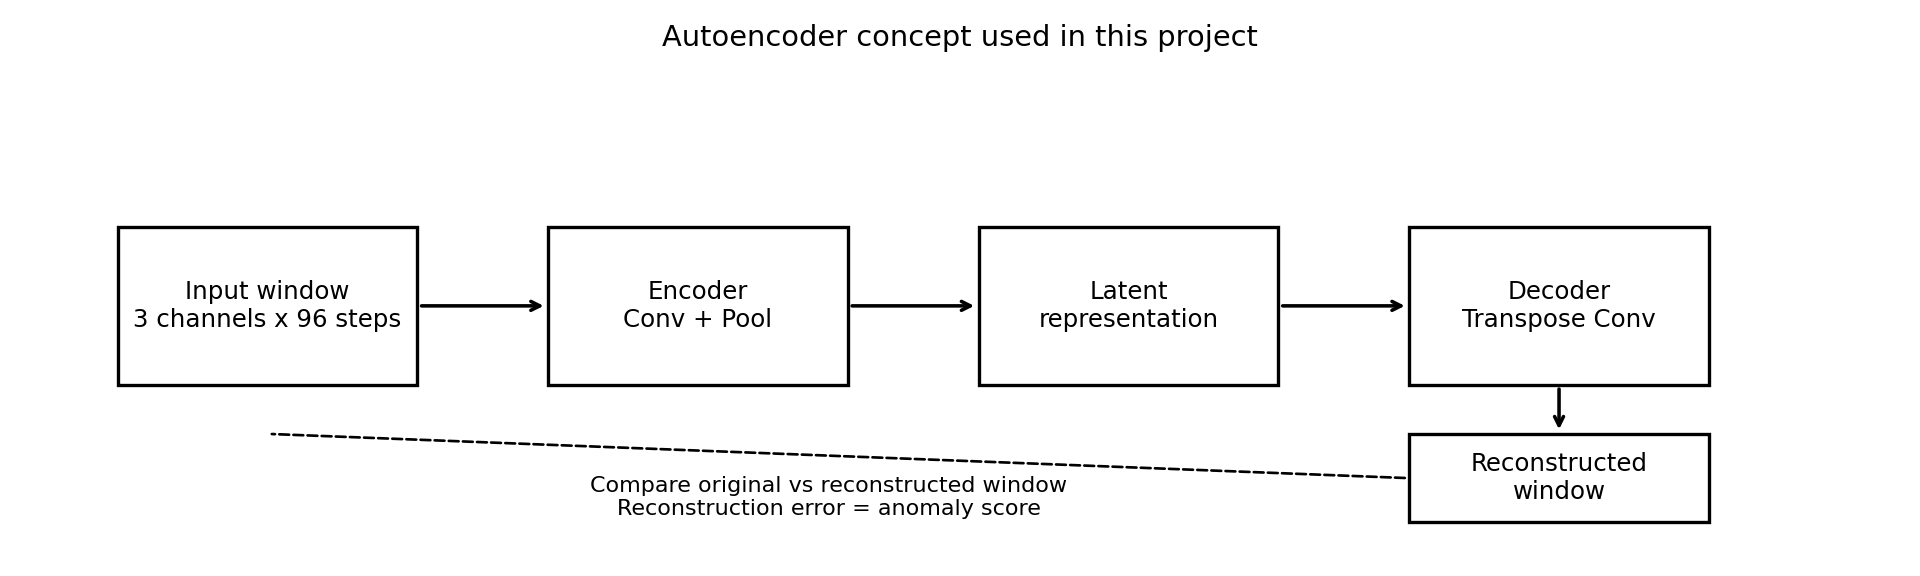
\includegraphics[width=\linewidth]{autoencoder_concept_diagram.png}
    \caption{Conceptual view of the reconstruction-based anomaly detector. A 24-hour window containing supply temperature, return temperature, and the flow channel is encoded, reconstructed, and scored by reconstruction error.}
    \label{fig:autoencoder_concept}
\end{figure}

\subsection{Clustering roles}

Two clustering roles were explored:

\begin{itemize}
\item operating-regime clustering on all windows, using summary statistics of each day
\item anomaly-only clustering on flagged windows, used as a secondary anomaly-family interpretation layer
\end{itemize}

The thesis should make clear that clustering is supportive rather than central in the final pipeline.

\begin{figure}[H]
    \centering
    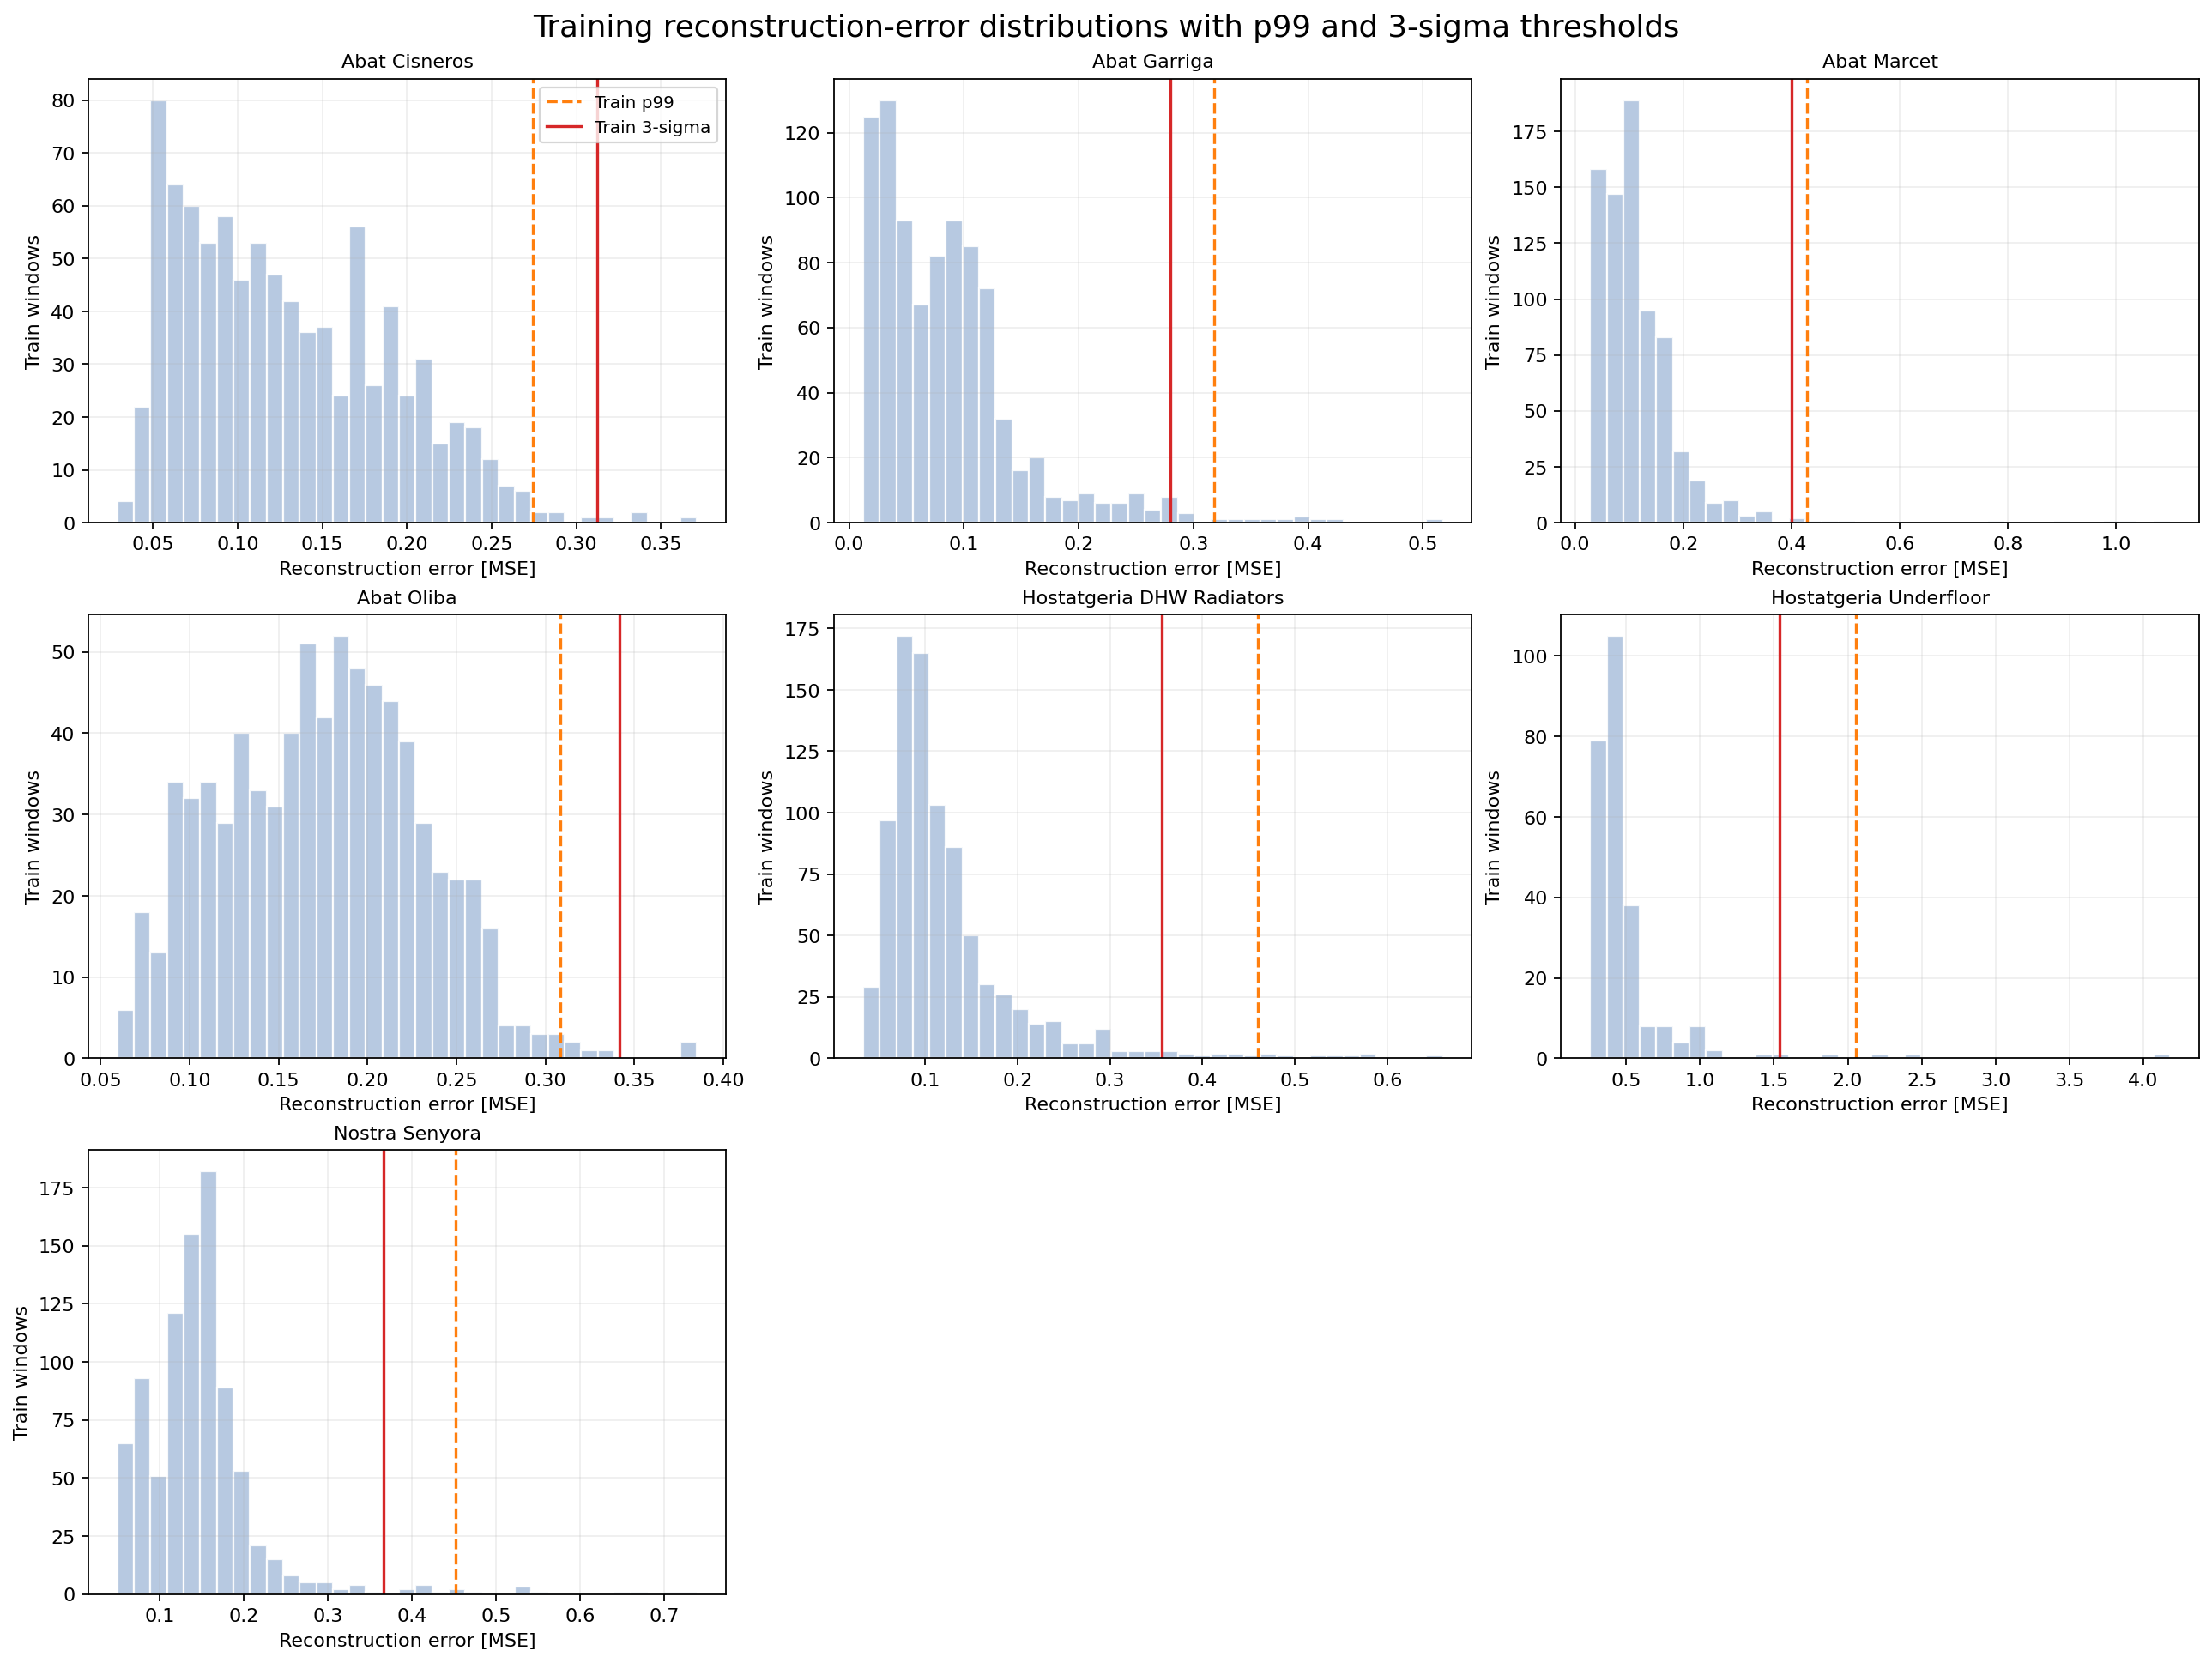
\includegraphics[width=\linewidth]{threshold_distribution_by_sheet_2026-06-07.png}
    \caption{Training reconstruction-error distributions for the modeled sheets, shown with both the training 99th percentile threshold and the 3-sigma threshold. The difference between the two thresholds depends on the shape and spread of the training reconstruction-error distribution.}
    \label{fig:threshold_distributions}
\end{figure}

\section{Results}

\subsection{Current main result set}

The current end-to-end result set used for the draft focuses on five heating-consumer sheets: Abat Cisneros, Abat Garriga, Abat Marcet, Abat Oliba, and Hostatgeria Underfloor. These five buildings were kept because they provided the most usable retained windows without the long faulty constant-value periods observed in two of the exploratory cases. The strongest anomaly case remains \texttt{cons\_hostatgeria\_underfloor\_hea}, while the five-building set as a whole still shows substantial variation in anomaly count, dominant feature, and engineering-baseline overlap.

\begin{table}[t]
\centering
\caption{Five-building result summary under the 3-sigma threshold.}
\label{tab:five_building_summary}
\begin{tabular}{lrrrr}
\toprule
Building & Windows & Flagged & Rate [\%] & Top feature \\
\midrule
Abat Cisneros & 1113 & 4 & 0.36 & Flow \\
Abat Garriga & 1107 & 17 & 1.54 & Return \\
Abat Marcet & 951 & 10 & 1.05 & Flow \\
Abat Oliba & 955 & 2 & 0.21 & Return \\
Hostatgeria Underfloor & 323 & 5 & 1.55 & Supply \\
\bottomrule
\end{tabular}
\end{table}

\begin{figure}[H]
    \centering
    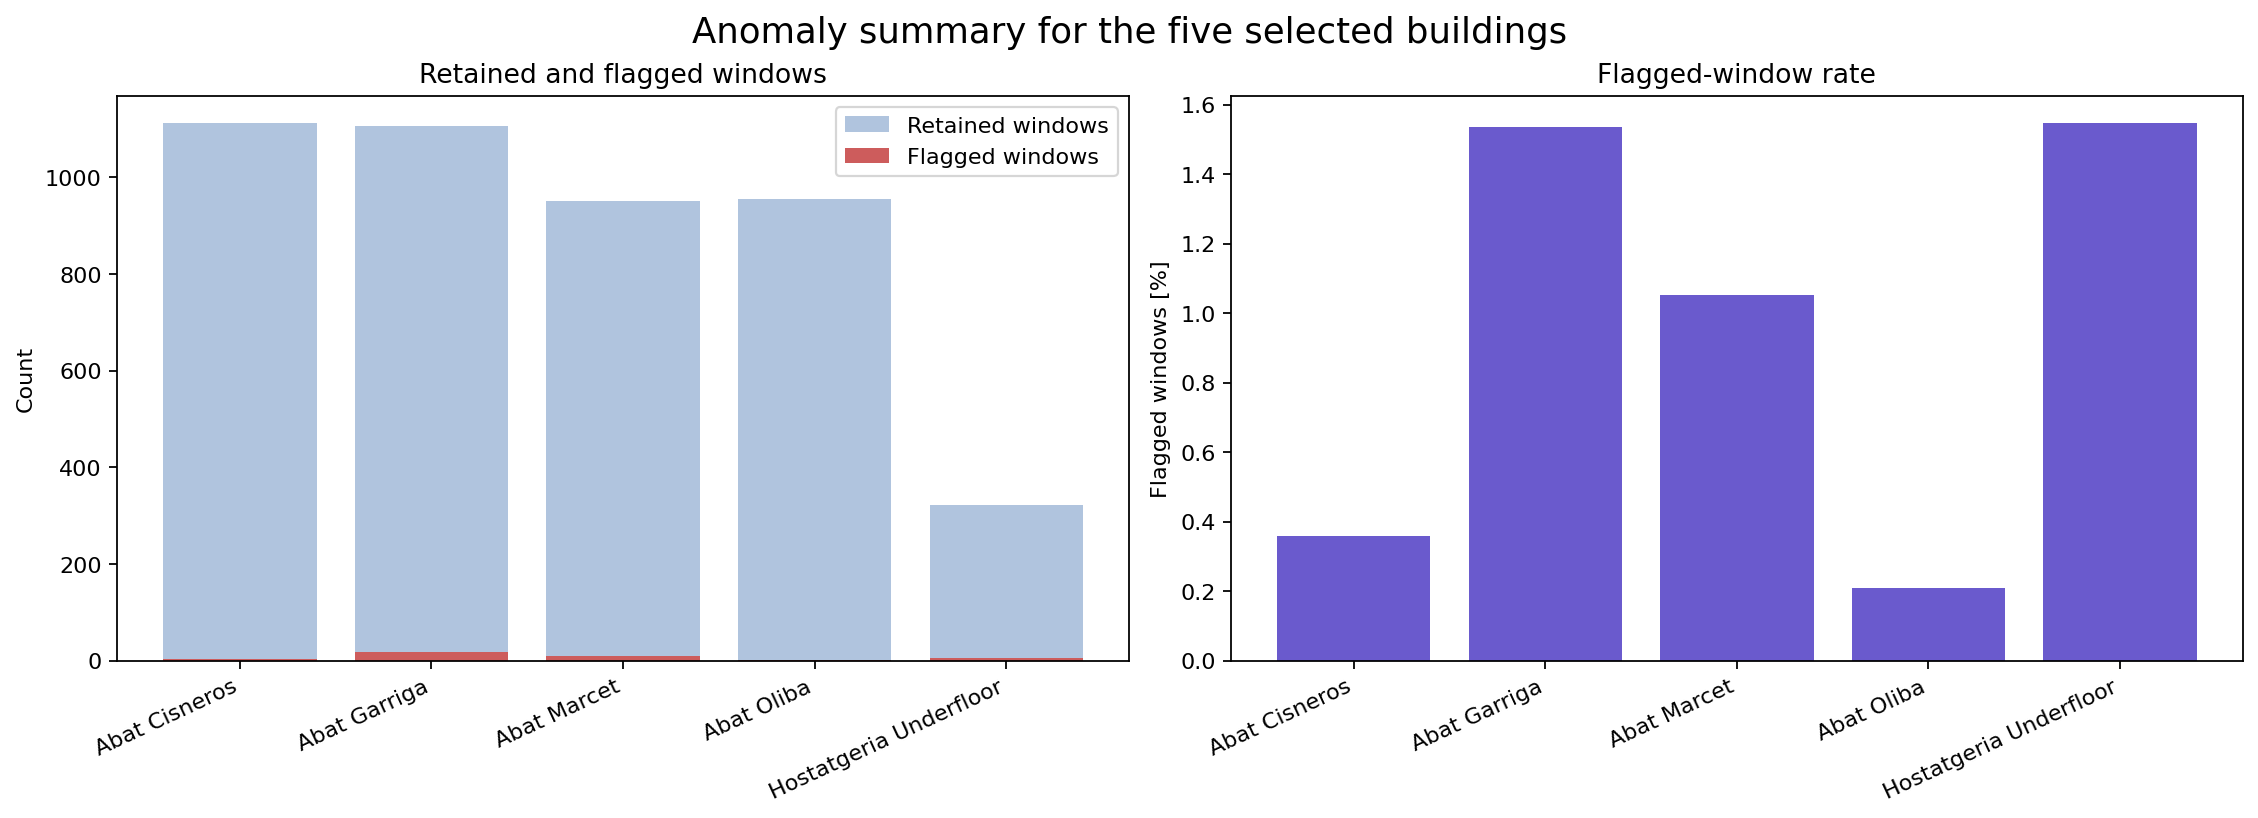
\includegraphics[width=\linewidth]{thesis_selected5_anomaly_summary.png}
    \caption{Retained-window count, flagged-window count, and flagged-window rate for the five selected buildings.}
    \label{fig:selected5_anomaly_summary}
\end{figure}

\begin{figure}[H]
    \centering
    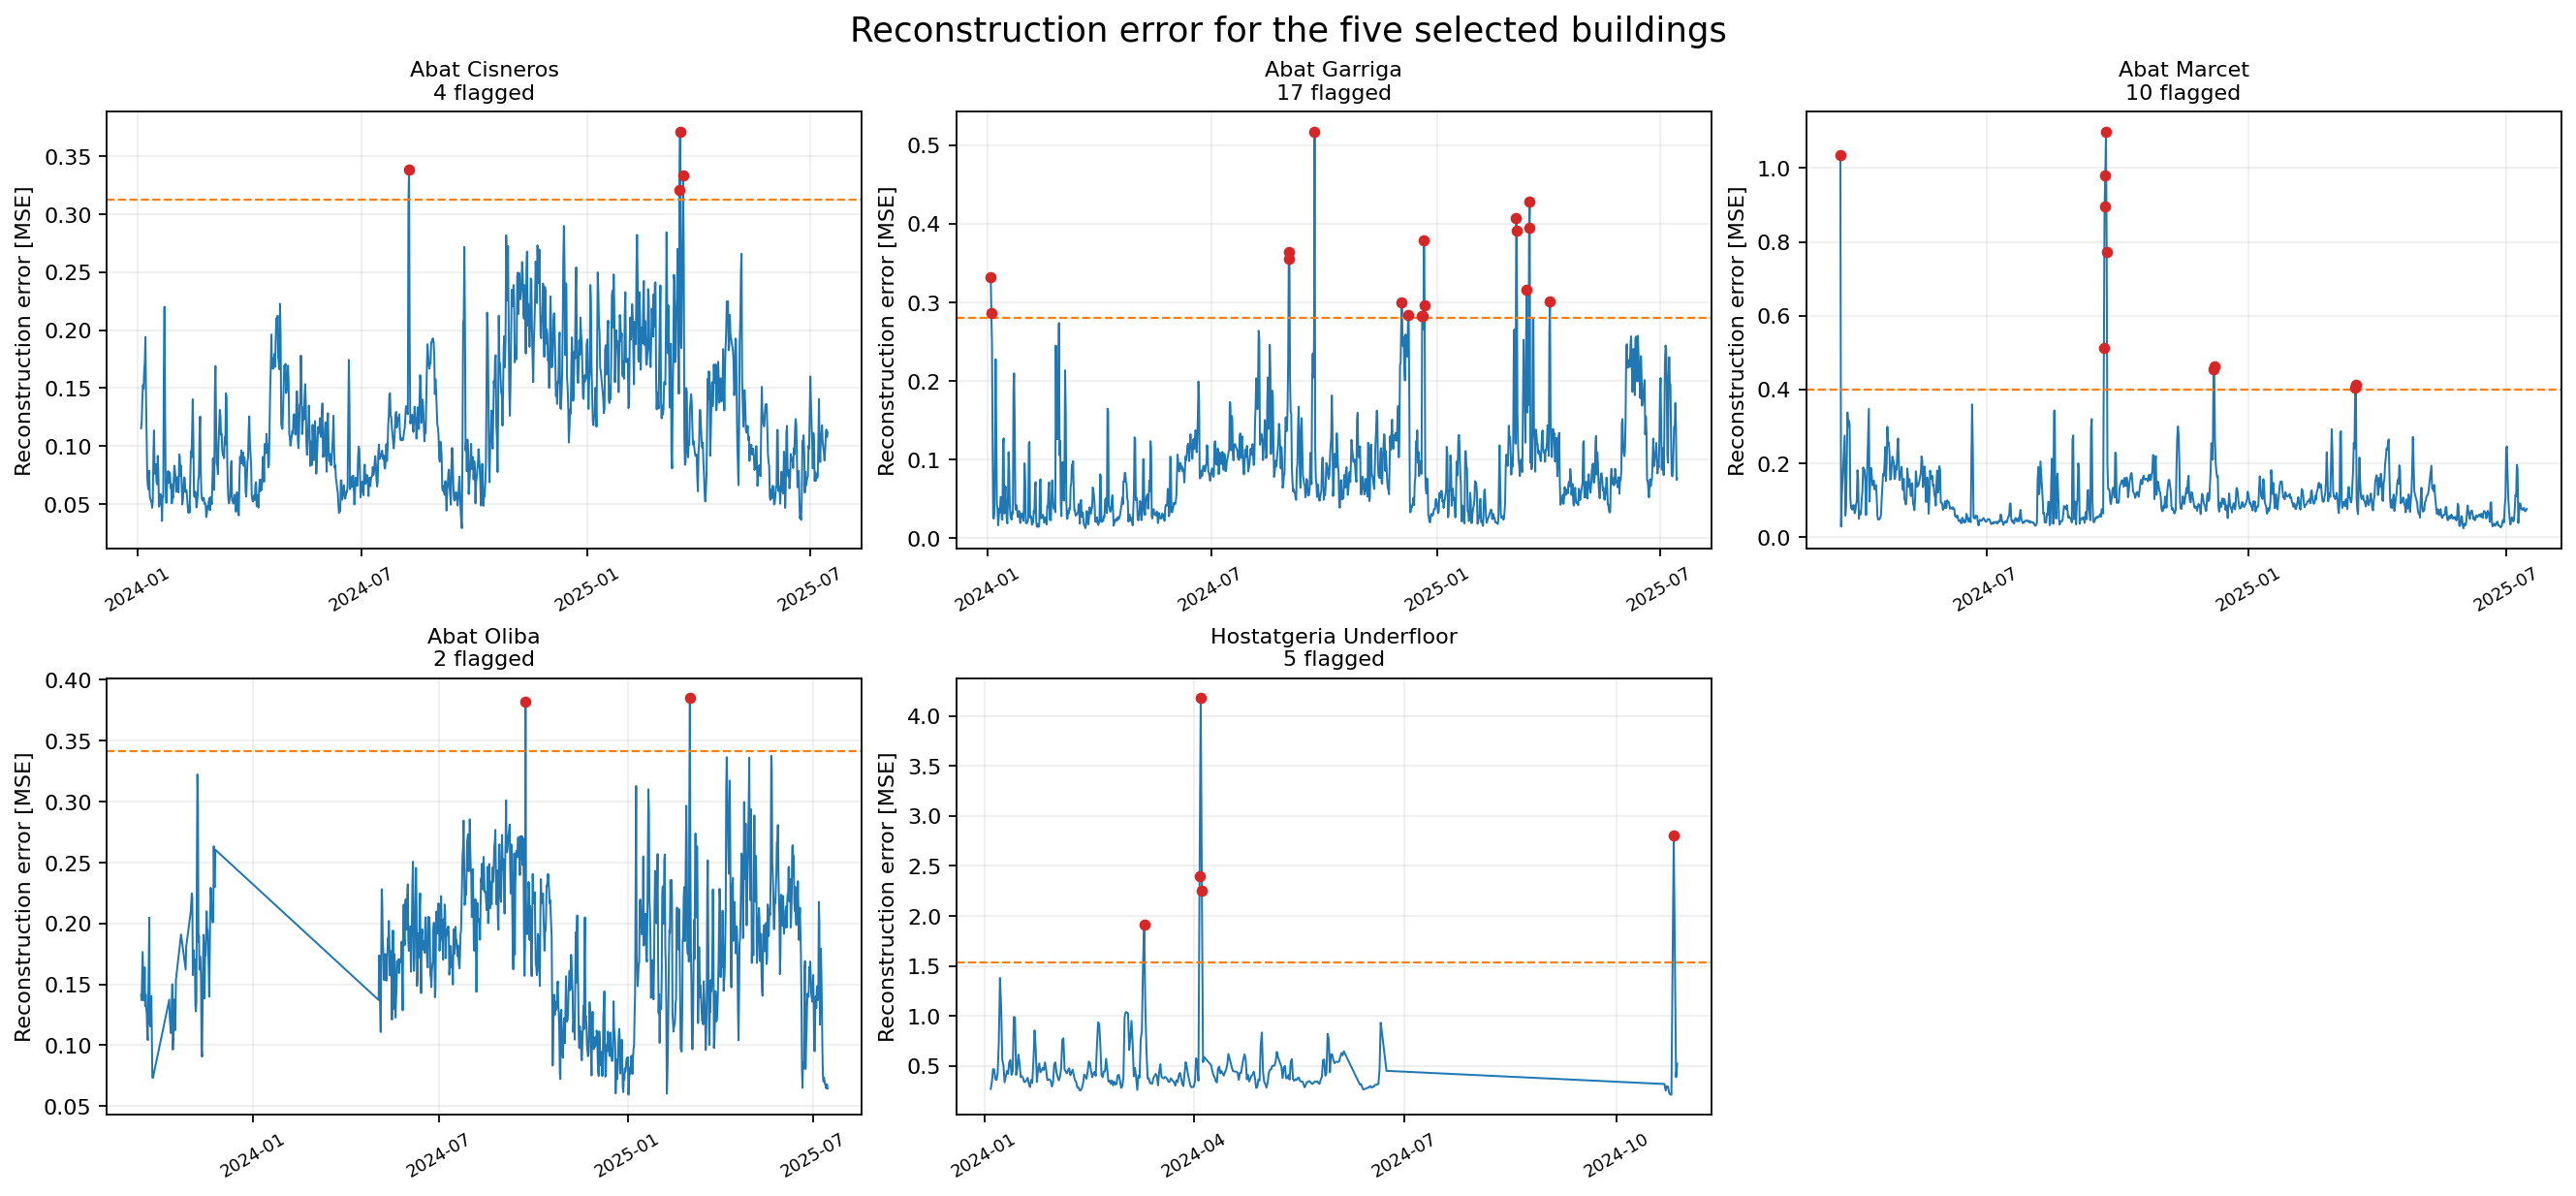
\includegraphics[width=\linewidth]{thesis_selected5_reconstruction_error_grid.png}
    \caption{Reconstruction-error timelines for the five selected buildings. The horizontal dashed line is the anomaly threshold and red points are flagged windows.}
    \label{fig:selected5_reconstruction_grid}
\end{figure}

\iffullfigures
\begin{figure}[H]
    \centering
    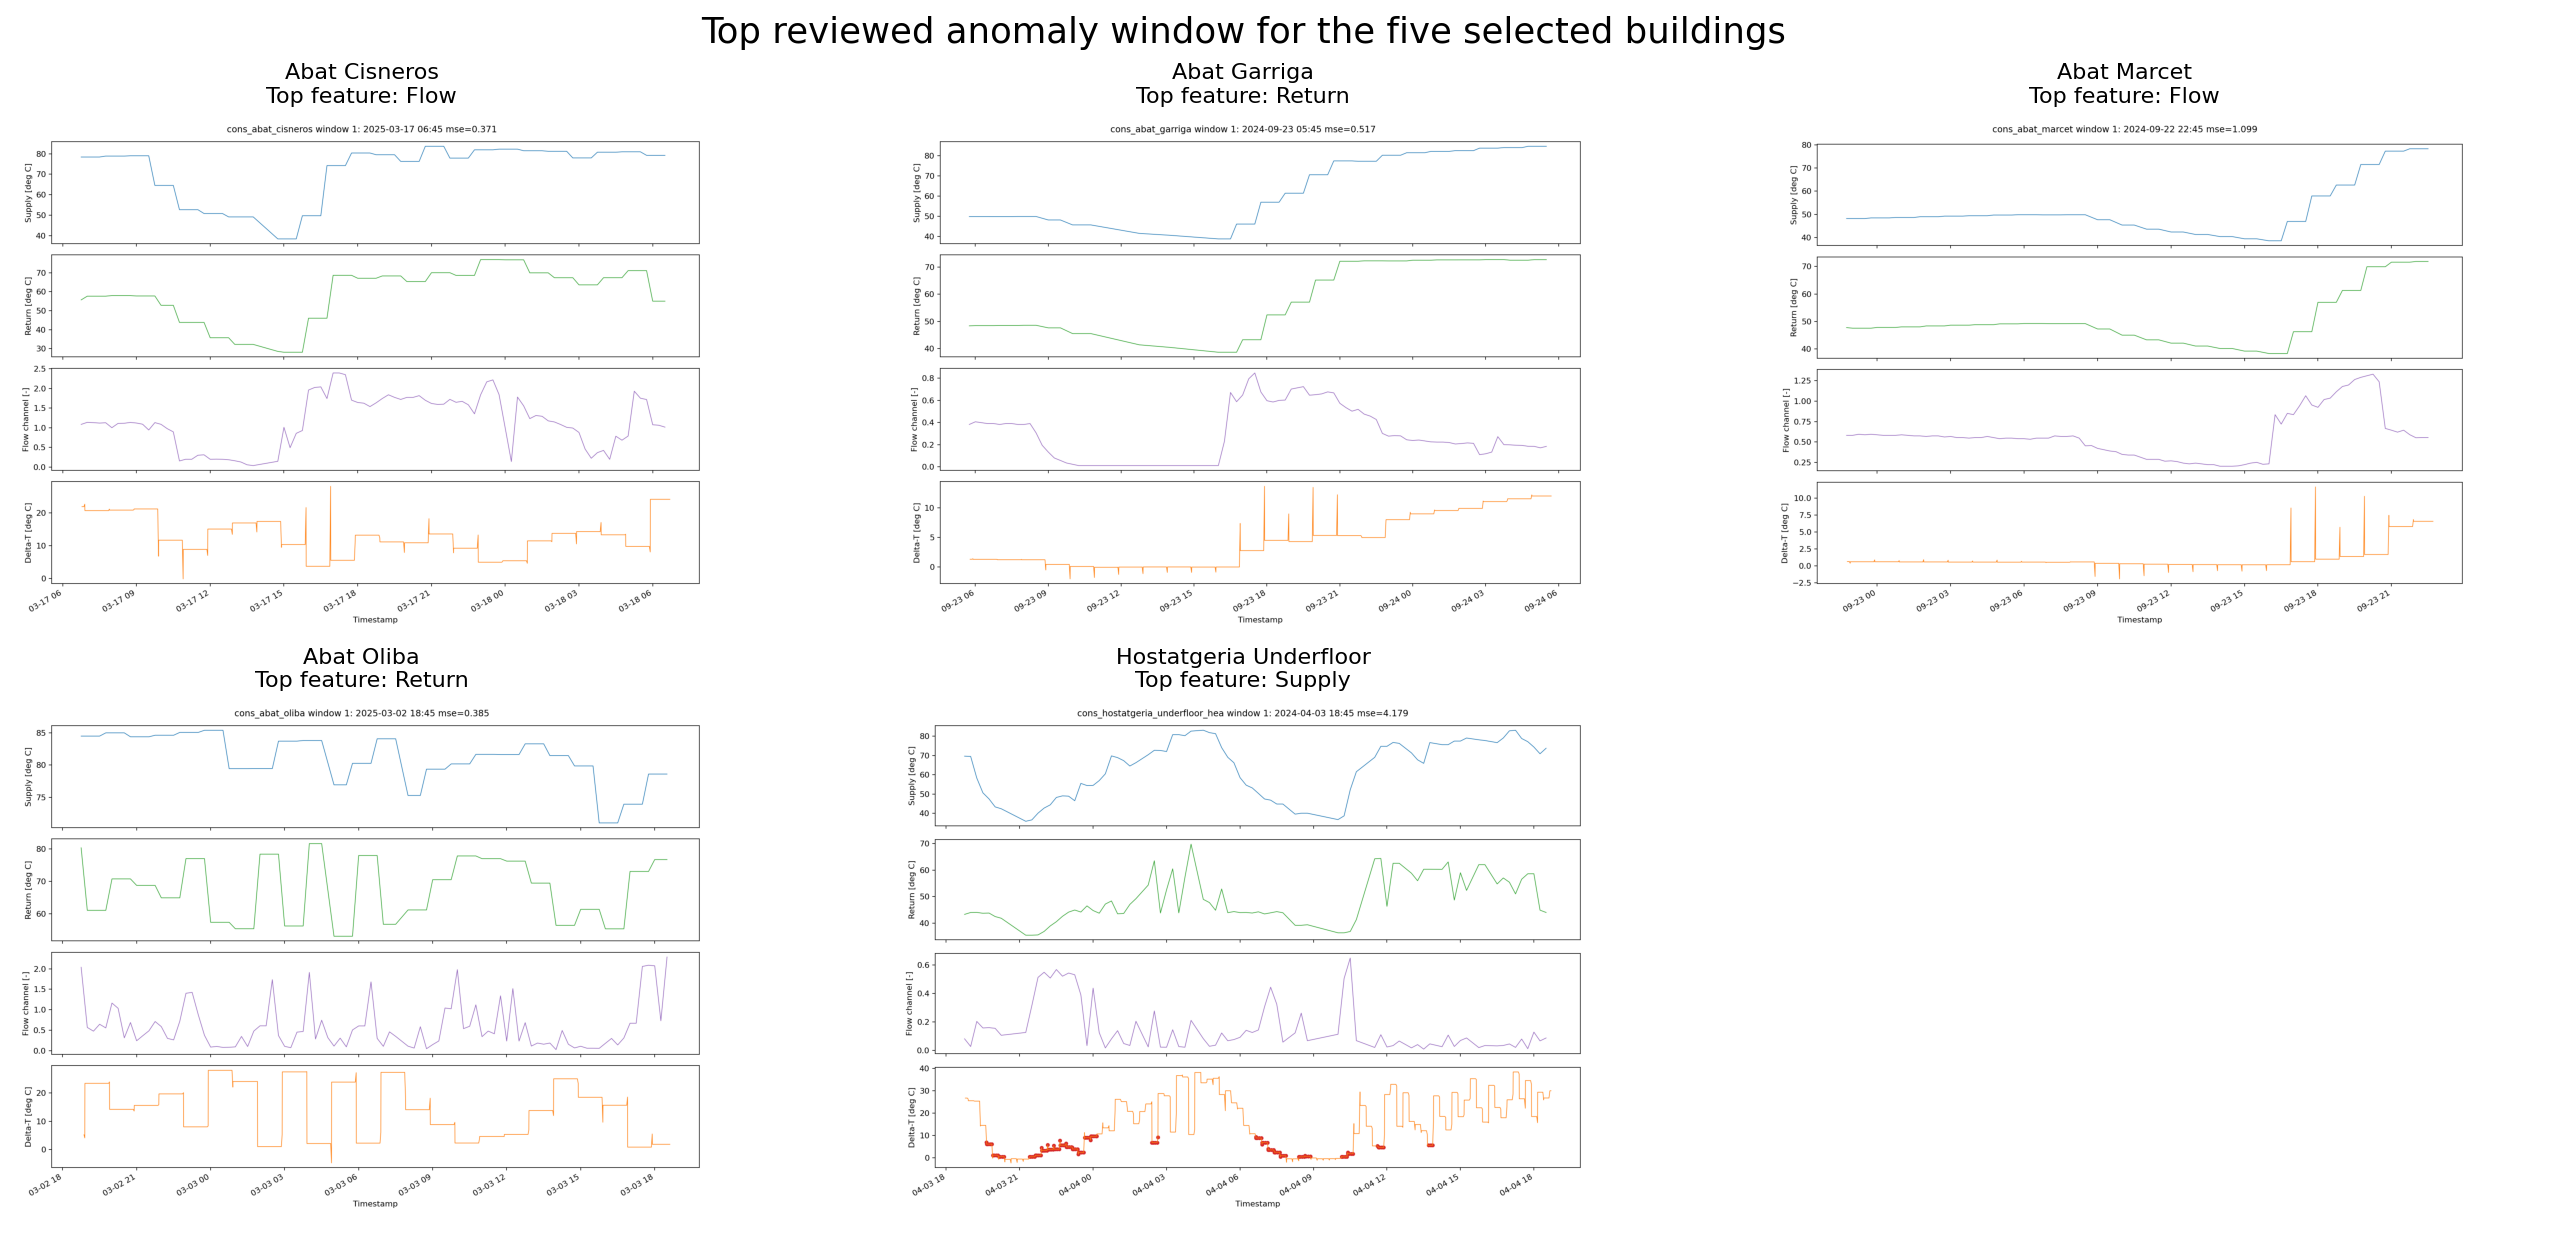
\includegraphics[width=\linewidth]{thesis_selected5_top_anomaly_grid.png}
    \caption{Top reviewed anomaly window for each of the five selected buildings. Each panel shows supply temperature, return temperature, the flow channel, and delta-T over the 24-hour anomaly window.}
    \label{fig:selected5_top_anomalies}
\end{figure}
\fi

\subsection{Dominant-feature interpretation}

The clearest current anomaly-typing view is the dominant-feature analysis. Across the five-building set, the anomalies are mainly flow-dominant and return-dominant, with Hostatgeria Underfloor providing the clearest supply-dominant case. This indicates that the autoencoder is detecting multiple anomaly families rather than only one repeated signature.

\begin{figure}[H]
    \centering
    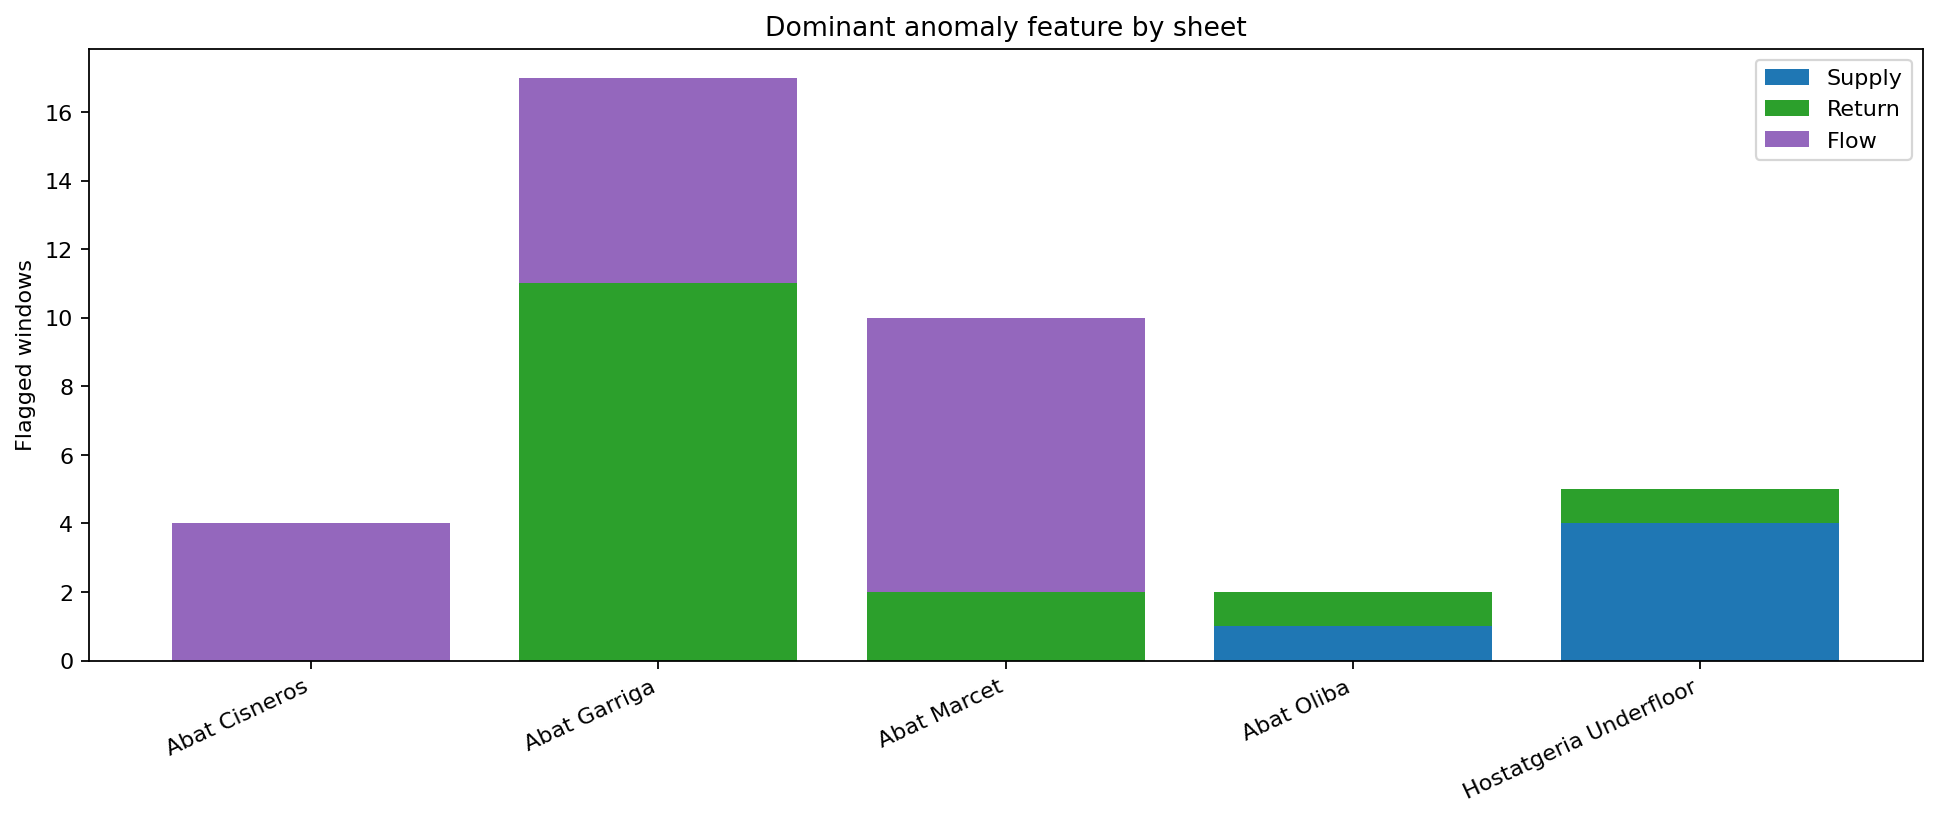
\includegraphics[width=\linewidth]{thesis_selected5_feature_type_by_sheet.png}
    \caption{Dominant anomaly feature by sheet for the five selected buildings.}
    \label{fig:selected5_feature_type}
\end{figure}

\iffullfigures
\begin{figure}[H]
    \centering
    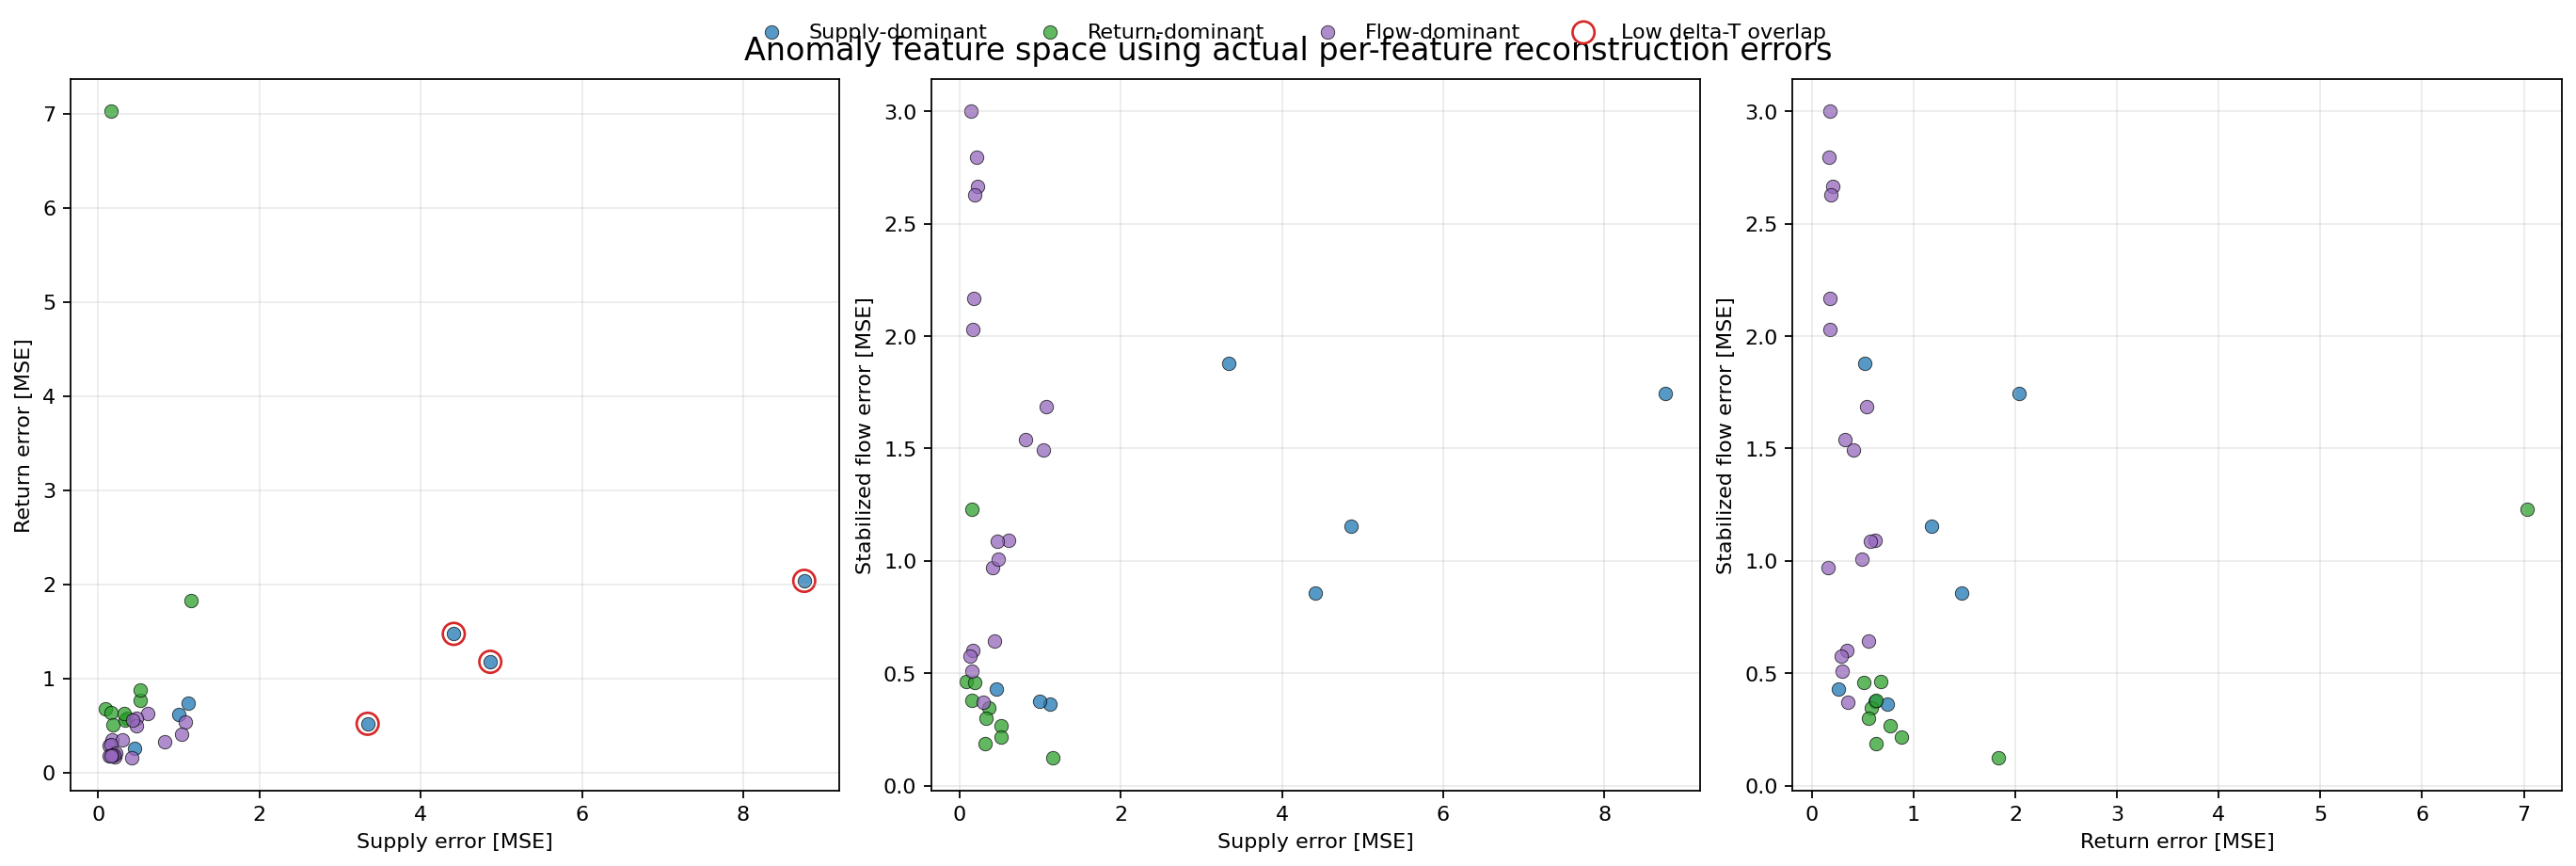
\includegraphics[width=\linewidth]{anomaly_feature_space_stabilized_log.png}
    \caption{Anomaly feature space using actual per-feature reconstruction errors. The axes are real feature-error quantities rather than PCA projections, and the point color indicates the dominant anomaly feature.}
    \label{fig:anomaly_feature_space}
\end{figure}
\fi

\subsection{Low delta-T overlap}

Only one sheet, \texttt{cons\_hostatgeria\_underfloor\_hea}, shows strong overlap between top reviewed autoencoder anomalies and the low delta-T baseline. This should be interpreted carefully. It makes underfloor heating the strongest validated case, but the absence of overlap in the other four buildings does not invalidate the autoencoder. It instead suggests that many detected anomalies are not low delta-T events and therefore require interpretation through dominant feature, flow-channel behavior, and domain review.

\begin{figure}[H]
    \centering
    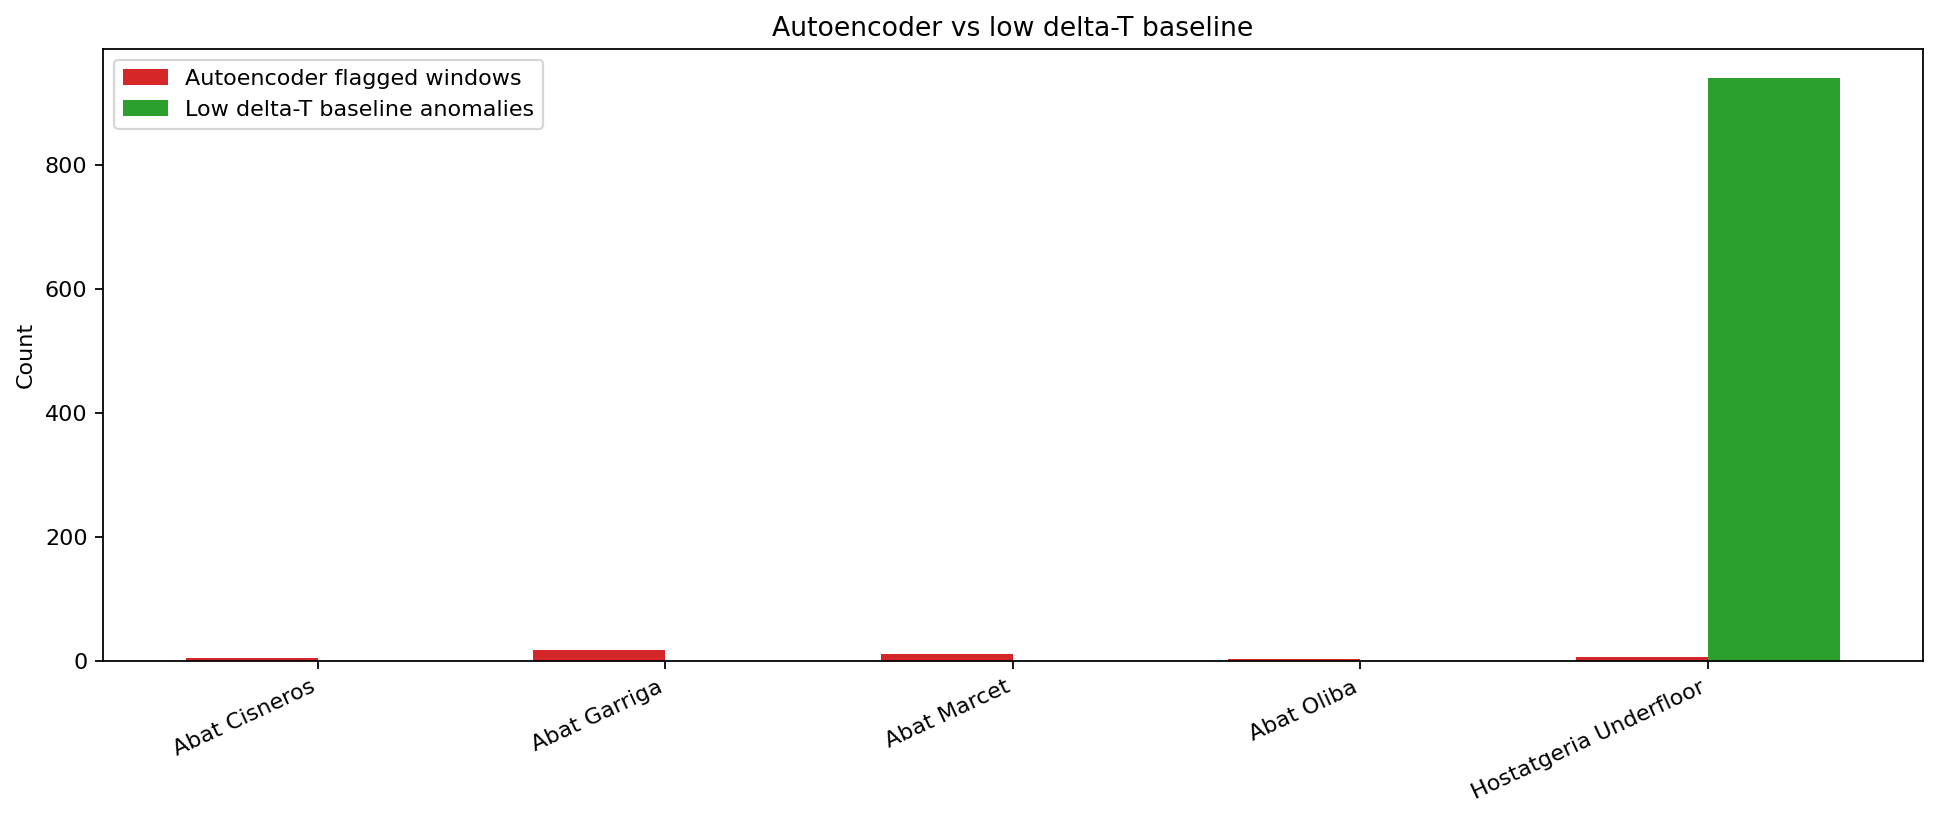
\includegraphics[width=\linewidth]{thesis_selected5_baseline_vs_autoencoder.png}
    \caption{Autoencoder anomaly counts compared with the engineering low delta-T baseline for the five selected buildings.}
    \label{fig:selected5_baseline_compare}
\end{figure}

\iffullfigures
\begin{figure}[H]
    \centering
    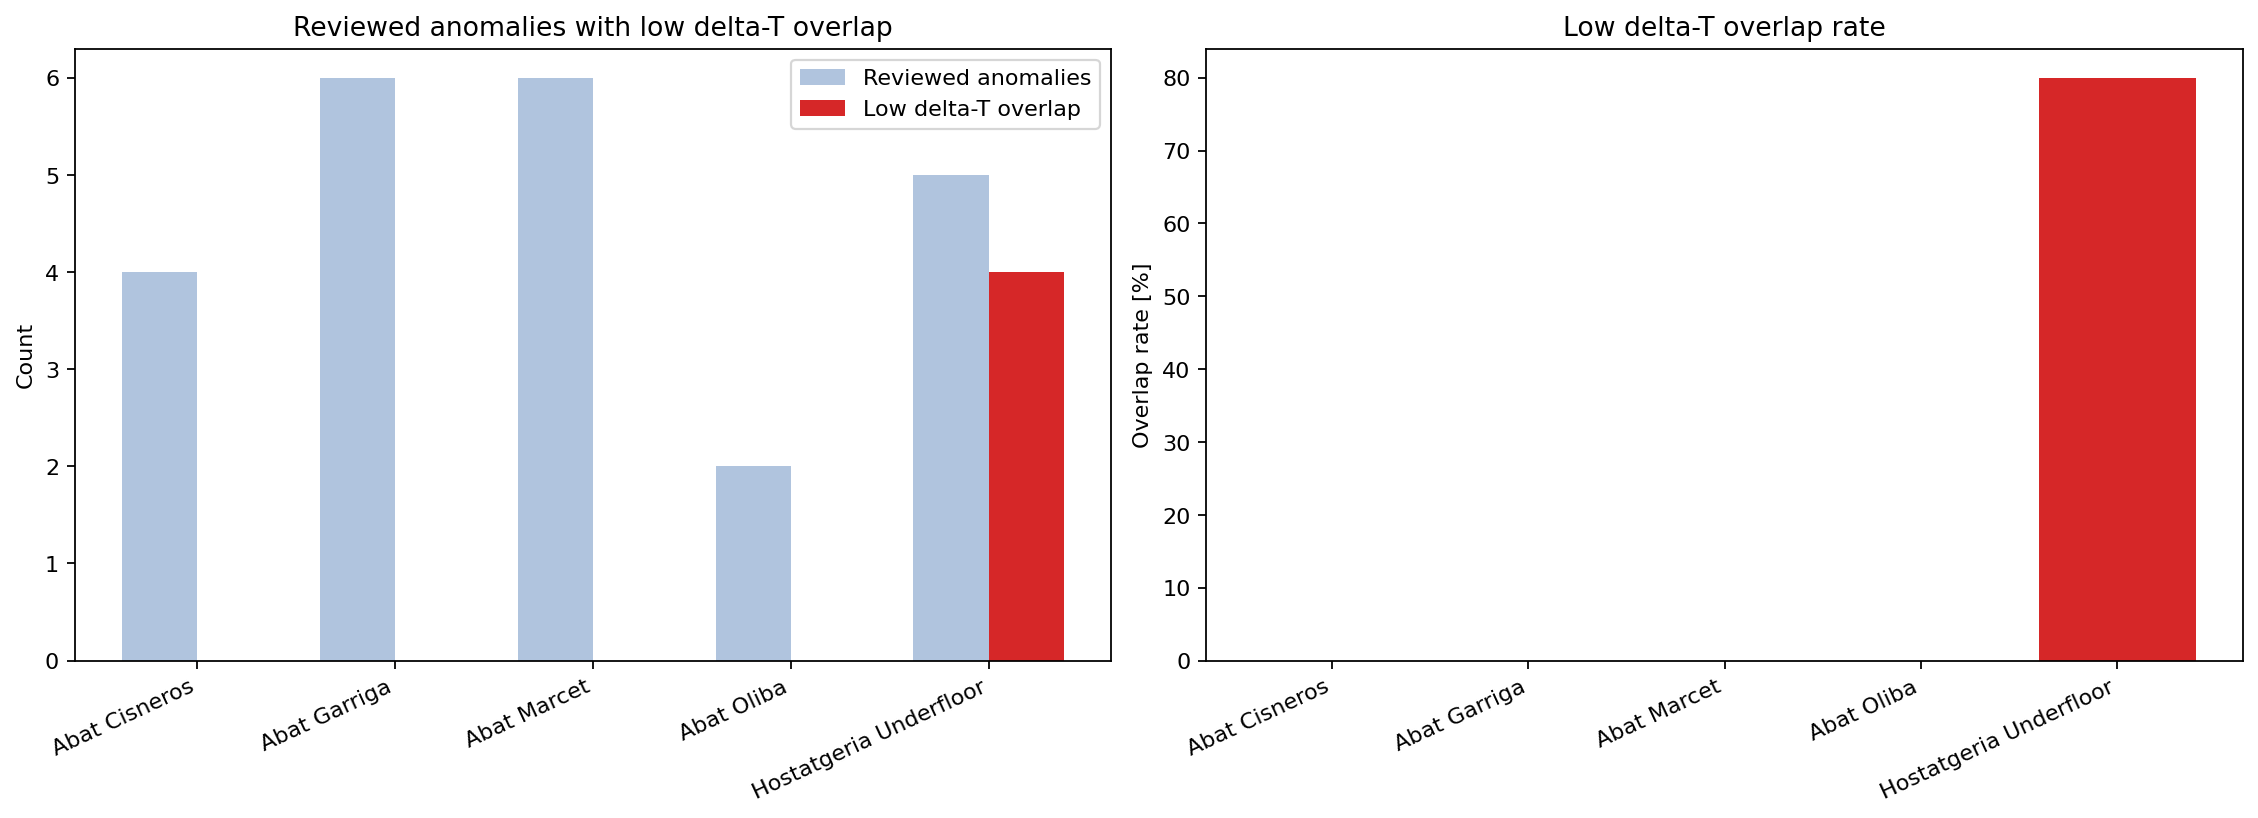
\includegraphics[width=\linewidth]{thesis_selected5_low_delta_overlap.png}
    \caption{Reviewed anomaly windows with low delta-T overlap and the corresponding overlap rate. Hostatgeria Underfloor is the only building with substantial overlap.}
    \label{fig:selected5_low_delta_overlap}
\end{figure}
\fi

\subsection{Operating regimes}

Operating-regime clustering indicates that daily windows do not form one undifferentiated population. Some sheets occupy very distinctive regimes, and regime occupancy is uneven. Underfloor heating stands out as the most distinctive operating-regime case. This supports the conclusion that its anomalies are associated with a coherent subsystem behavior rather than random variation.

\iffullfigures
\begin{figure}[H]
    \centering
    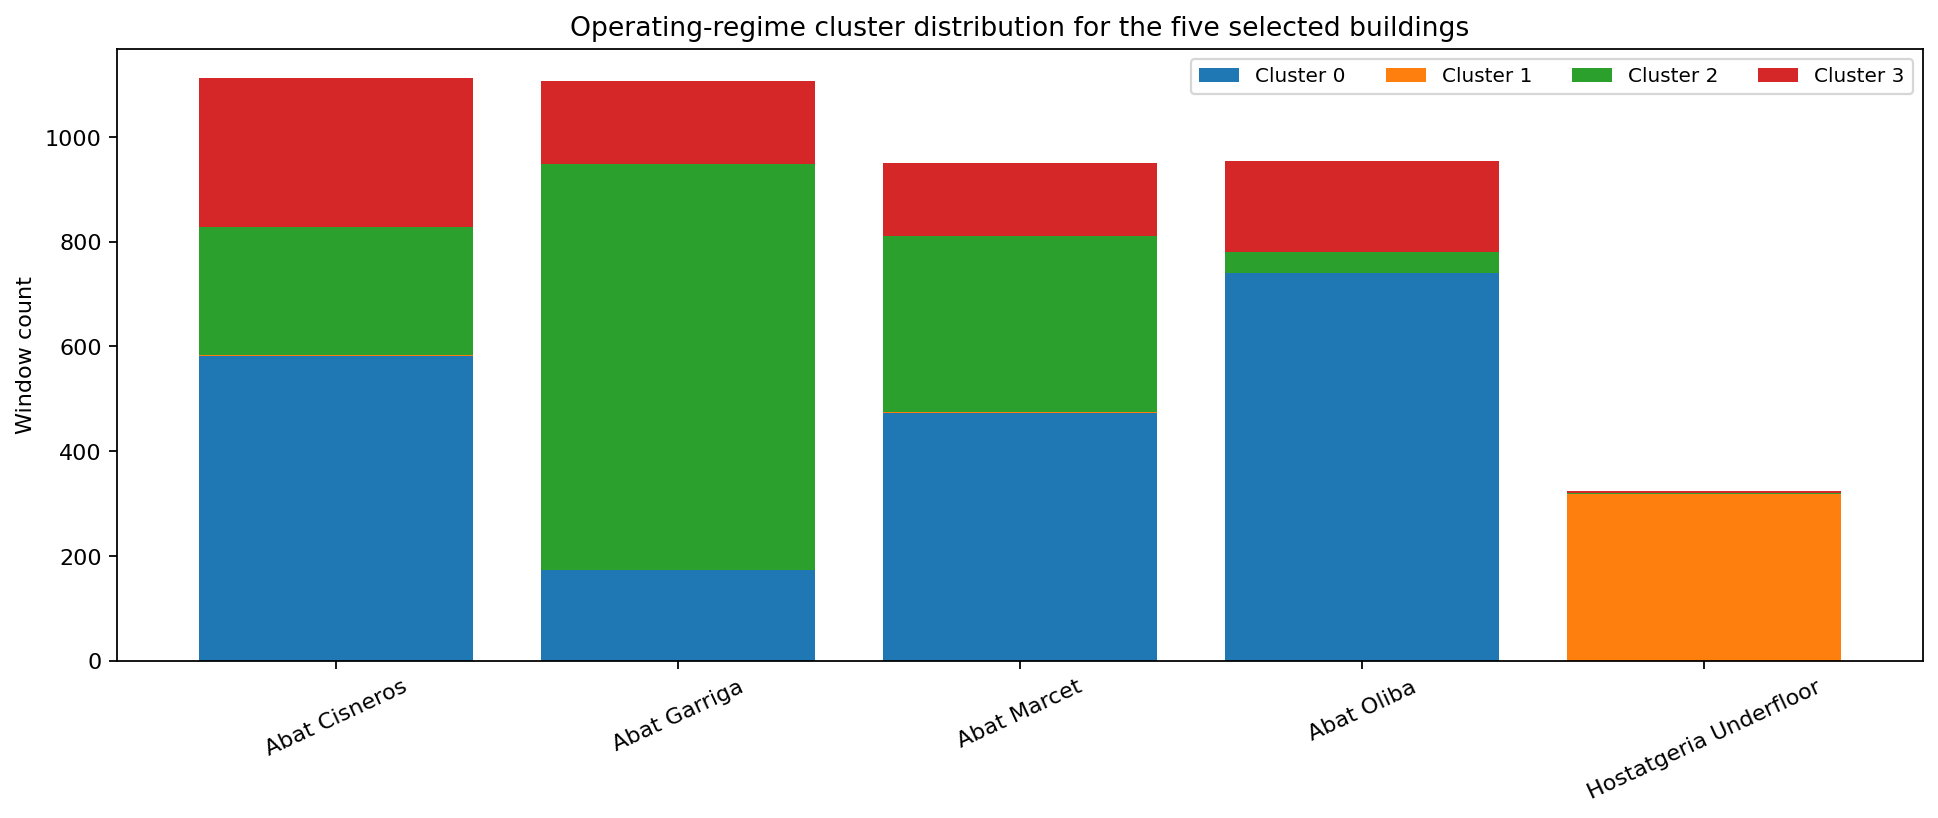
\includegraphics[width=\linewidth]{thesis_selected5_window_cluster_distribution.png}
    \caption{Operating-regime cluster distribution for the five selected buildings. The interpretation should focus on the fact that occupancy is uneven and that underfloor heating occupies a distinctive regime, rather than on the cluster labels themselves.}
    \label{fig:operating_regimes}
\end{figure}
\fi

\subsection{Threshold comparison}

The comparison between p99 and 3-sigma shows that threshold choice materially affects anomaly counts. The effect is sheet-dependent rather than global: some sheets become more selective under 3-sigma, while others become less selective. This is a useful result in itself because it shows that the training-error distribution shape must be considered when choosing an anomaly threshold.

\begin{figure}[H]
    \centering
    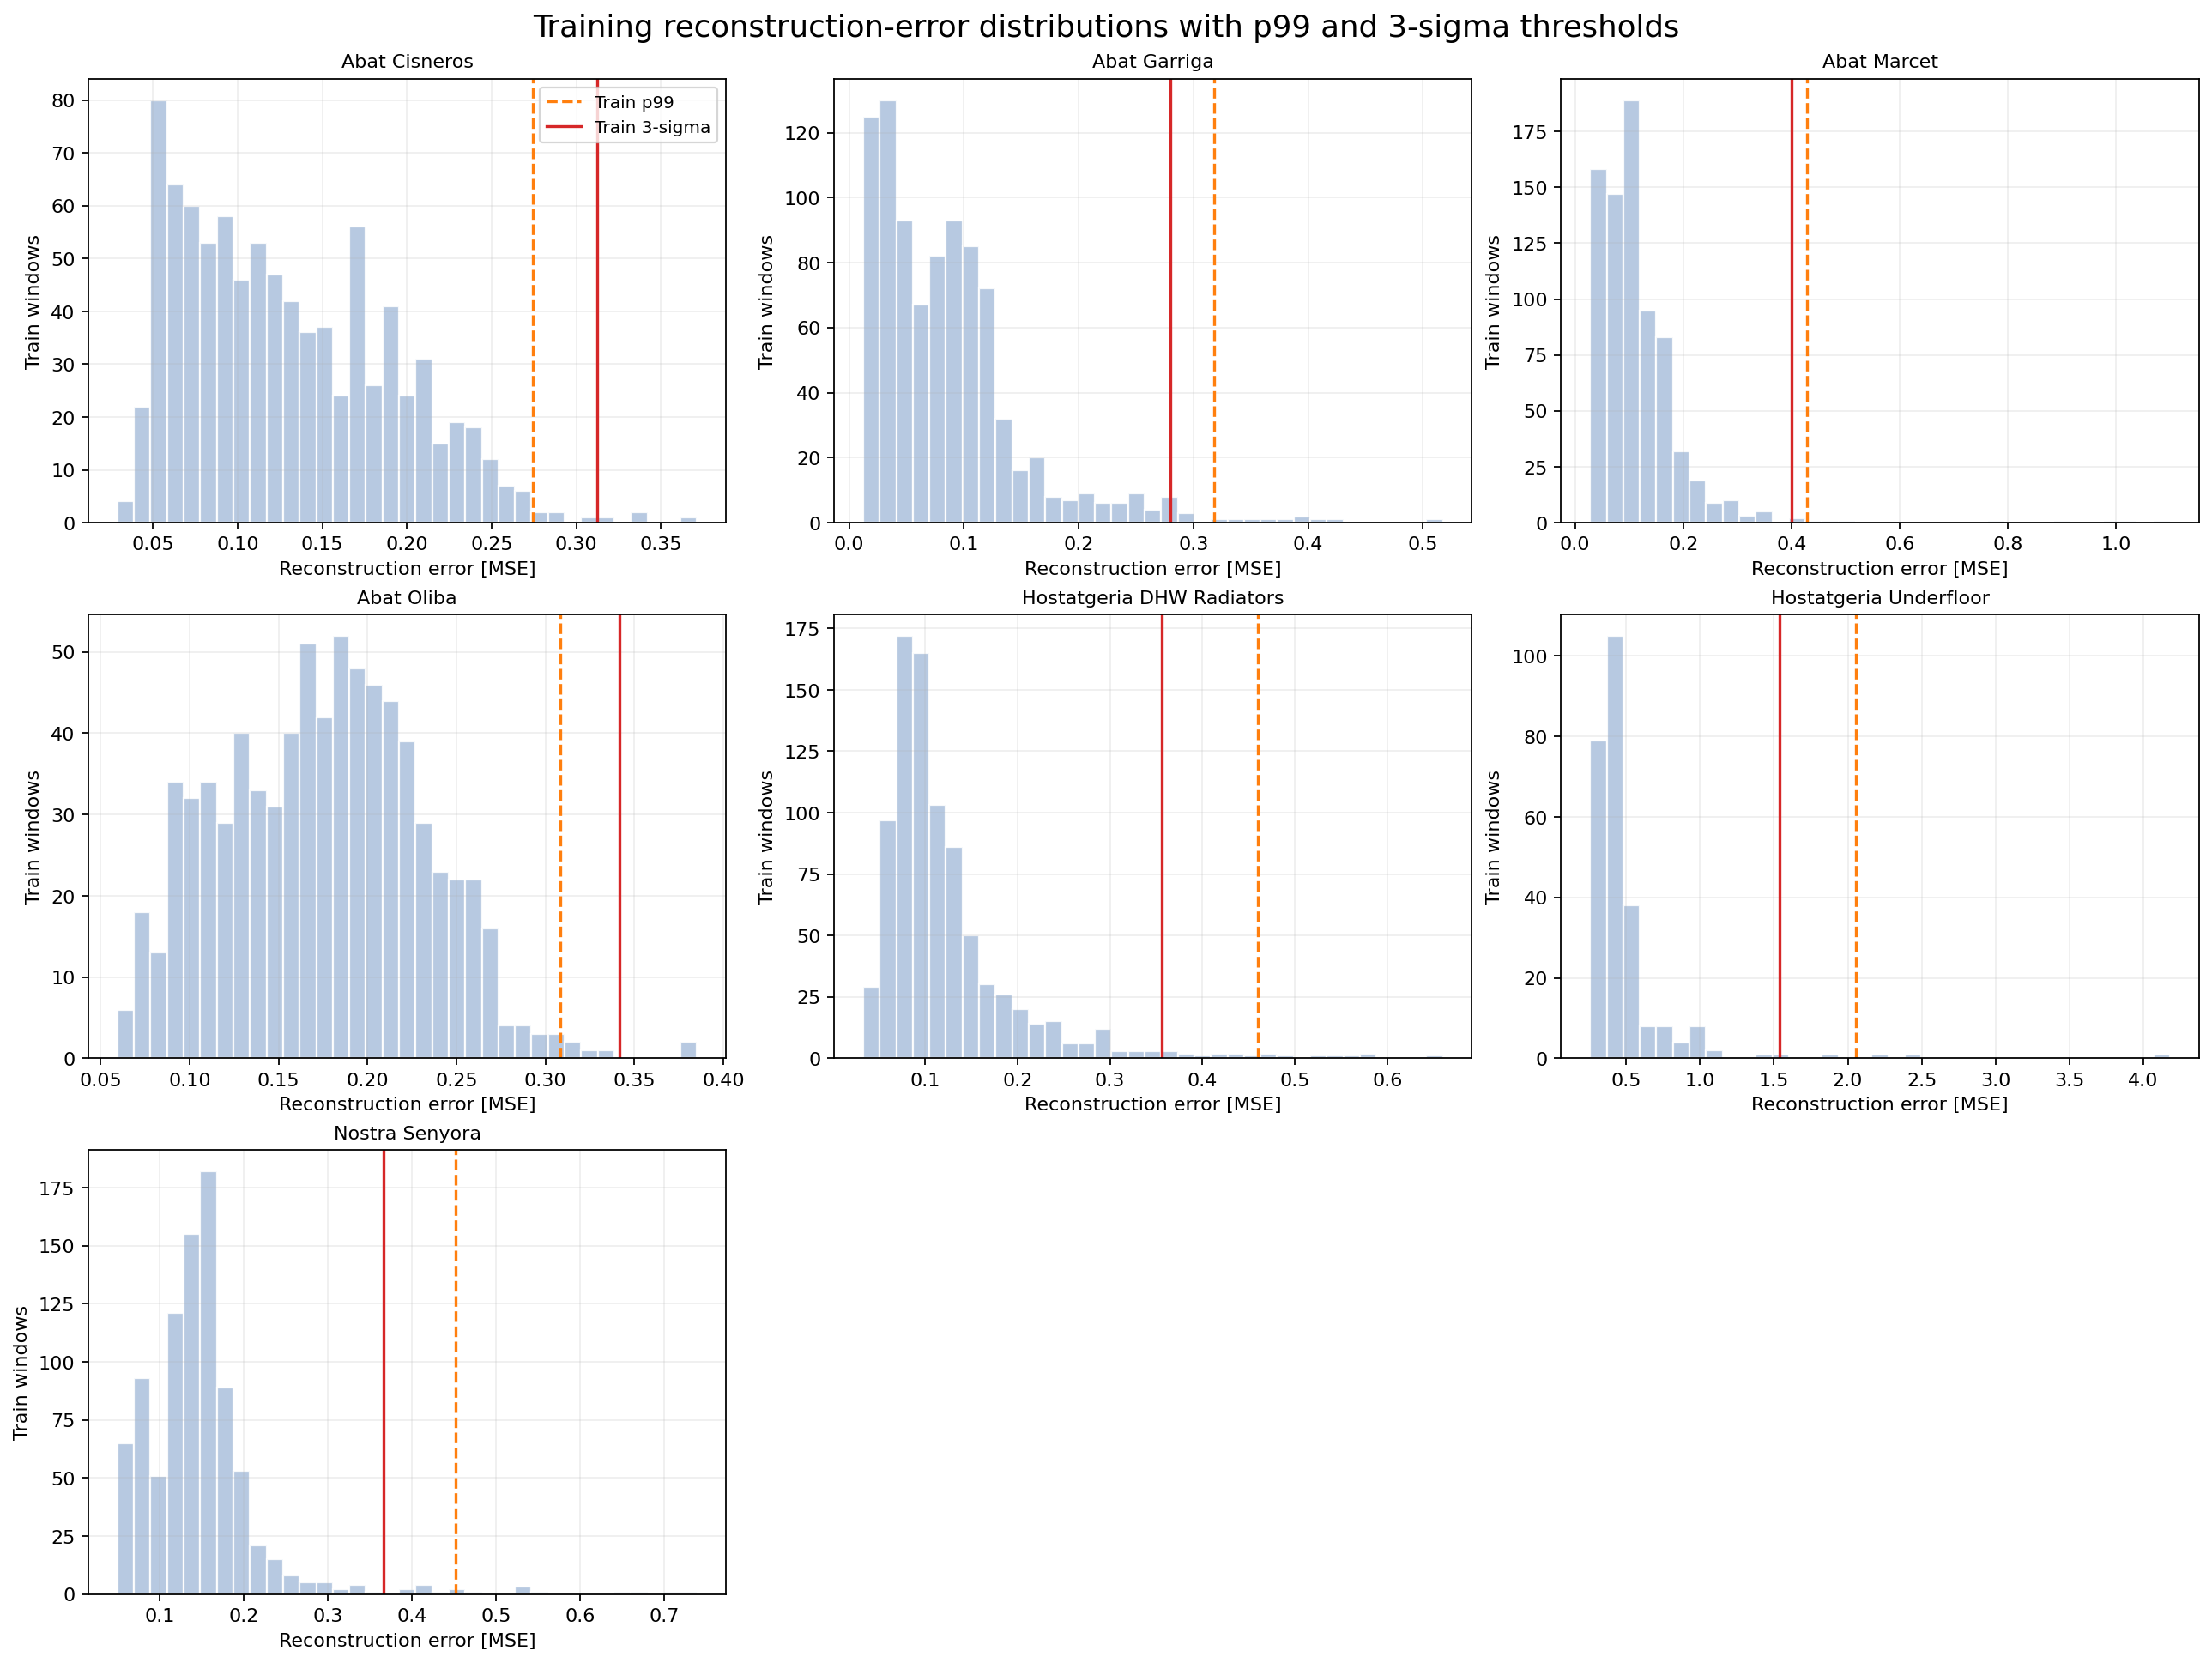
\includegraphics[width=\linewidth]{threshold_distribution_by_sheet_2026-06-07.png}
    \caption{Training reconstruction-error distributions with the p99 and 3-sigma thresholds overlaid.}
    \label{fig:threshold_result_view}
\end{figure}

\subsection{Flow-channel sensitivity comparison}

During model development, the anomaly counts were found to be sensitive to how the flow channel was represented. The clearest example is \texttt{cons\_abat\_oliba}, where the direct raw-flow version produced windows dominated by very small delta-T and inflated flow values, while the final flow-channel representation yielded anomalies that were more interpretable in terms of supply or return behavior.

\iffullfigures
\begin{figure}[H]
    \centering
    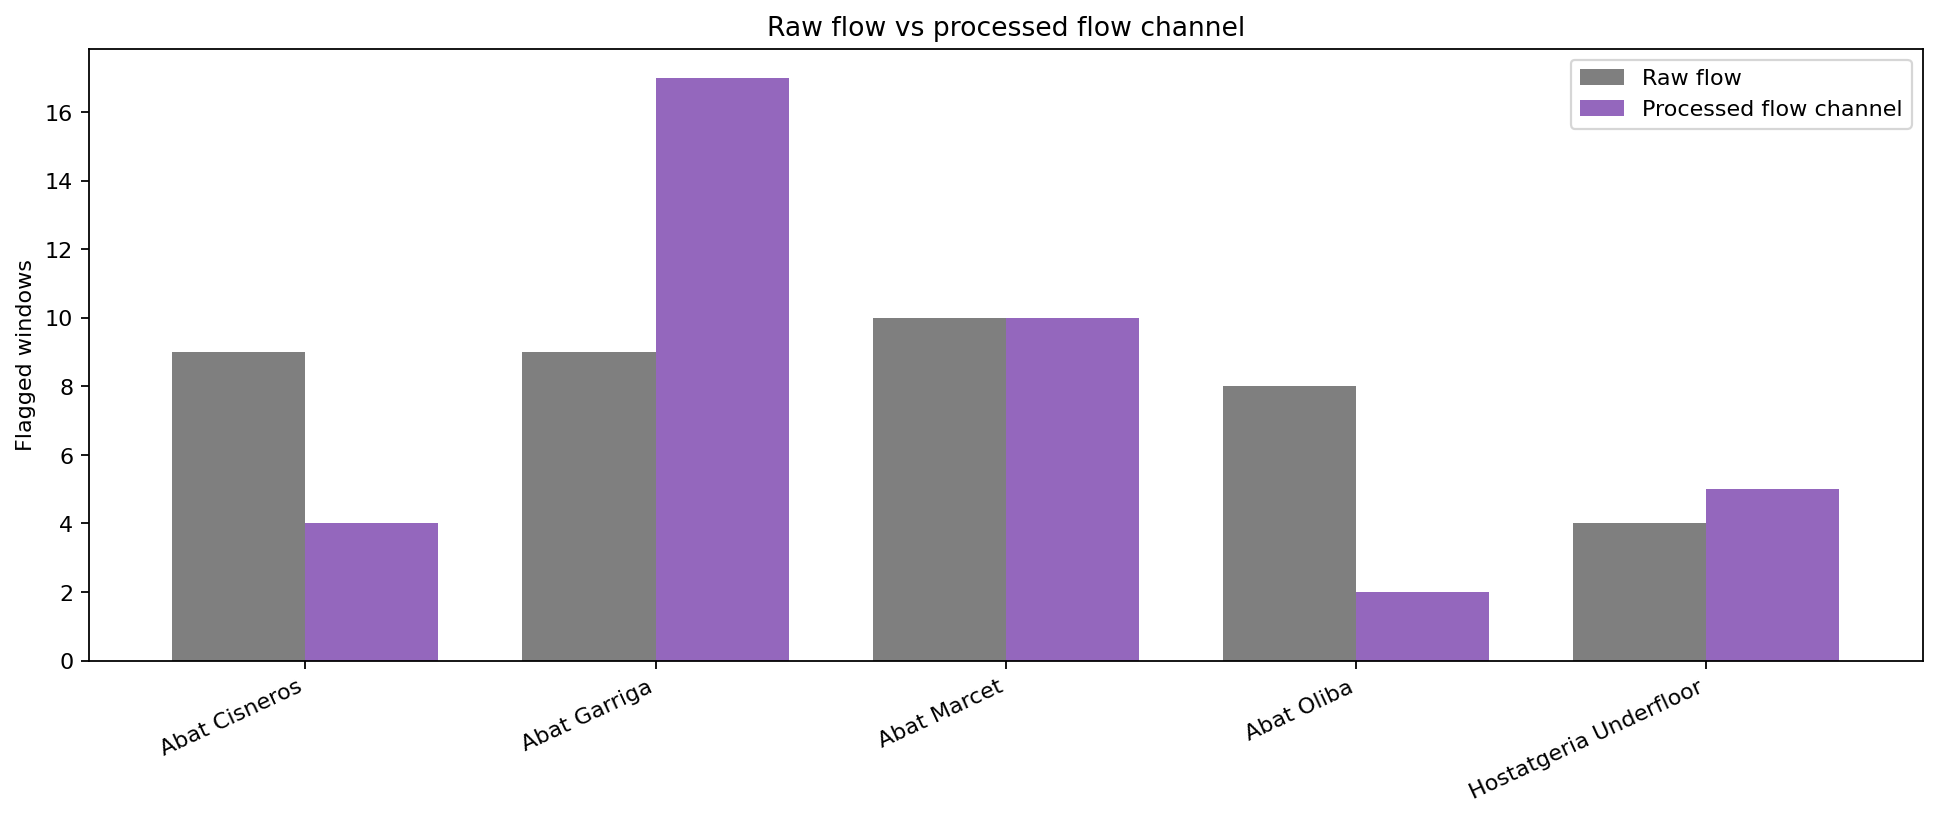
\includegraphics[width=\linewidth]{thesis_selected5_raw_vs_processed_counts.png}
    \caption{Flagged anomaly counts for raw-flow and final flow-channel representations. The comparison is kept here as a sensitivity analysis for the draft.}
    \label{fig:flow_channel_sensitivity}
\end{figure}
\fi

\iffullfigures
\begin{figure}[H]
    \centering
    
\includegraphics[width=0.48\linewidth]{inspect_autoencoder_cons_abat_oliba_01.png}
    \hfill
    
\includegraphics[width=0.48\linewidth]{inspect_autoencoder_cons_abat_oliba_stabilized_log_01.png}
    \caption{Abat Oliba top anomaly under the raw-flow representation (left) and the final flow-channel representation (right). This pair is retained in the draft because it is the clearest visual justification for the final flow-channel choice, even if only one representation will be emphasized in the final thesis version.}
    \label{fig:abat_oliba_flow_compare}
\end{figure}
\fi

\subsection{Train-test split and anomaly timing}

The anomalies are not confined to the first chronological portion of the data. Some buildings show both training and later test-period anomalies, which is useful when thinking about eventual live deployment.

\iffullfigures
\begin{figure}[H]
    \centering
    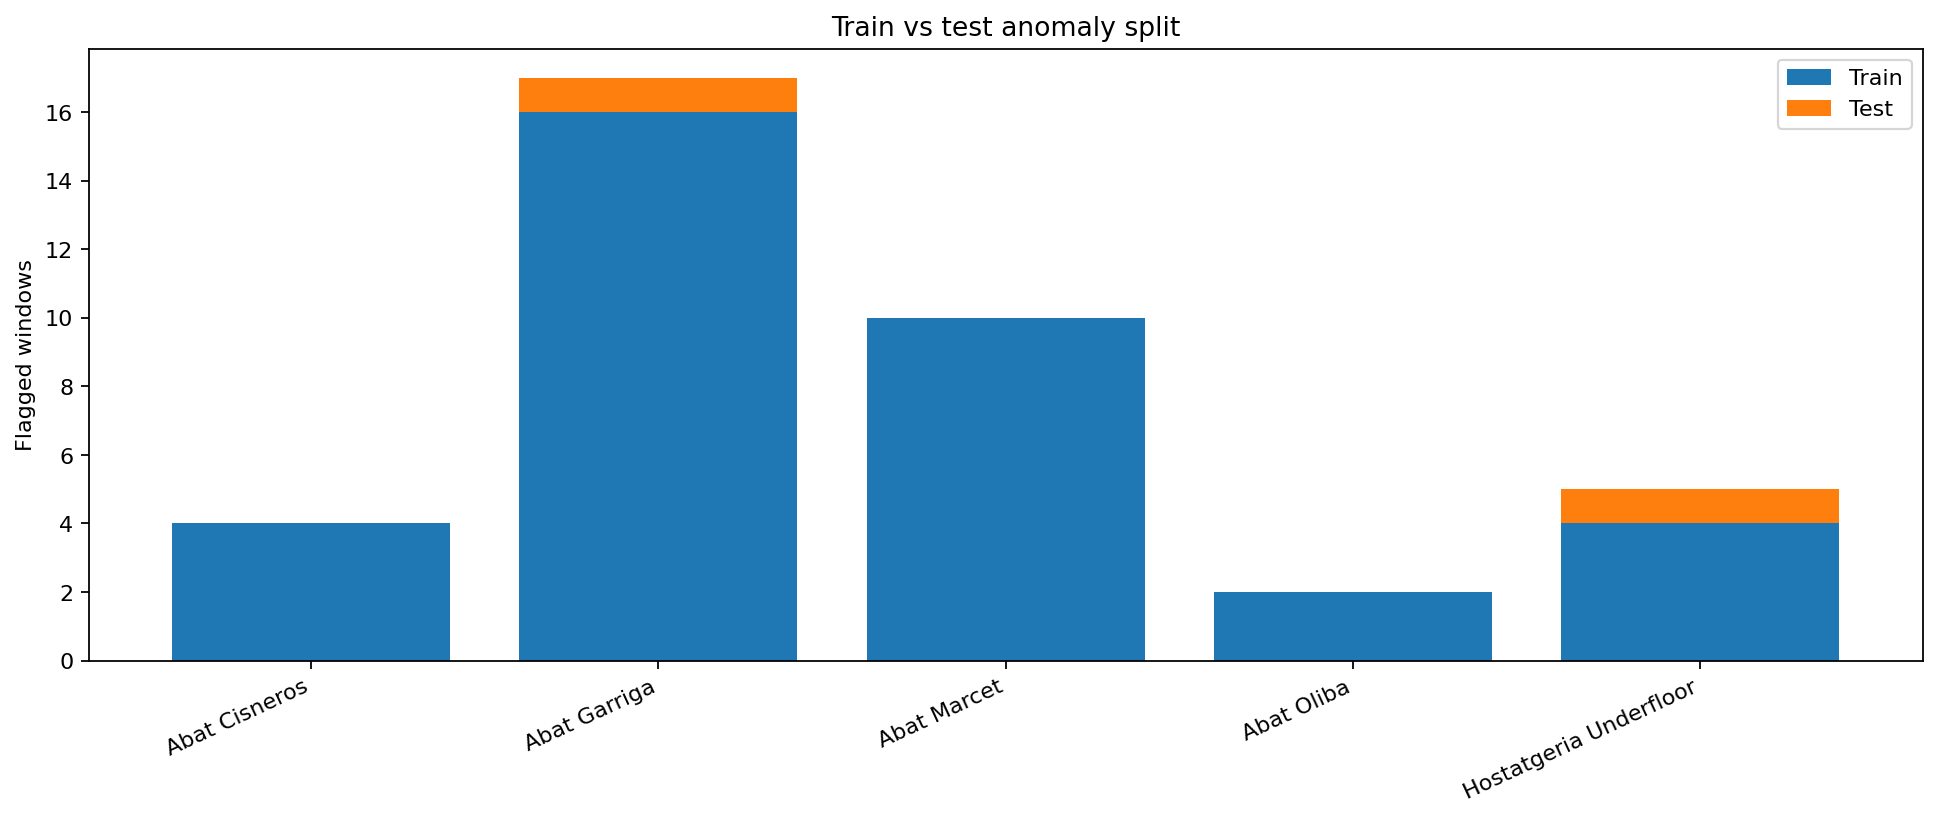
\includegraphics[width=\linewidth]{thesis_selected5_train_vs_test_split.png}
    \caption{Train versus test anomaly split for the five selected buildings.}
    \label{fig:selected5_train_test}
\end{figure}
\fi

\section{Discussion}

\subsection{What is currently convincing}

The most convincing current conclusion is that reconstruction-based anomaly detection is viable for this dataset and that \texttt{cons\_hostatgeria\_underfloor\_hea} provides a strong thesis case. It is physically distinctive, it overlaps the engineering baseline, and its anomaly patterns remain interpretable under both raw and stabilized flow views.

\subsection{What remains uncertain}

The biggest remaining limitation is still validation. Most sheets do not have labeled faults, so anomaly interpretation depends on triangulation:

\begin{itemize}
\item reconstruction error
\item dominant feature
\item signal plots
\item low delta-T overlap
\item supervisor and domain review
\end{itemize}

This means the thesis should frame most anomalies as credible candidates rather than confirmed faults.

\subsection{Implications for live deployment}

The historical result pack is already useful for deployment preparation. Once one to two months of live data become available, the intended strategy is to apply the historical-trained detector prospectively and evaluate the flagged windows through operational review rather than standard classification metrics.

\subsection{Writing priorities}

When drafting the final thesis, the narrative should remain focused. The autoencoder is the main method. The low delta-T baseline is the main engineering comparison. Dominant-feature attribution is the main anomaly interpretation layer. Clustering should be presented as a supporting analysis rather than the core detection method.

\section{Conclusion}

This thesis develops a reconstruction-based anomaly-detection pipeline for a small district-heating network with limited fault labels. The work adapts ideas from the HEAT paper to a setting where long historical coverage is more useful than large-scale peer-group clustering. The current results show that the method can identify interpretable anomalous operating windows and that the strongest case is underfloor heating, where the detected anomalies also align with a simple engineering low delta-T rule.

The broader seven-sheet analysis shows that anomaly behavior is heterogeneous across the network. Flow-dominant anomalies are the most common, return-dominant anomalies are the second main group, and supply-dominant anomalies are less frequent. Stabilized flow improves interpretability relative to raw flow and is therefore the main reporting lens. Operating-regime clustering remains useful for context, but dominant-feature attribution is the more effective explanation layer.

The next stage of the work is to apply the current detector to live data and use that prospective period as an operational evaluation step. This will help determine whether the anomaly candidates identified in historical data correspond to meaningful ongoing system behavior.


\begin{acks}
The acknowledgments section should be finalized once the supervisor, collaborators, and external contributors to the project are confirmed.
\end{acks}

\bibliographystyle{ACM-Reference-Format}
\bibliography{references}

\appendix
\section{Writing notes}

This appendix can be replaced later with:

\begin{itemize}
\item additional figures
\item threshold comparison tables
\item supervisor review artifacts
\item extended anomaly examples
\end{itemize}


\label{pg:lastPageofMainmatter}

% Disable the template back-cover and DiVA export pages in the working draft
% to keep Overleaf compilation reliable on the free plan.
% \cleardoublepage
% \clearpage\thispagestyle{empty}\mbox{}
% \kthbackcover
% \fancyhead{}
% \section*{\texteuro\texteuro\texteuro\texteuro\@ For DIVA \texteuro\texteuro\texteuro\texteuro}
% \lstset{numbers=none}
% \divainfo{pg:lastPageofMainmatter}

\end{document}
